\documentclass[doc,11pt,donotrepeattitle]{apa7}

% --- Idioma y tipografía ---
\usepackage[spanish,es-noquoting,es-tabla]{babel}
\usepackage{fontspec}
\usepackage{csquotes}

% --- Formato de página ---
\geometry{margin=2.54cm}
\usepackage{setspace}
\onehalfspacing

% --- Contenido ---
\usepackage{amsmath}
\usepackage{booktabs}
\usepackage{graphicx}
\usepackage{longtable}
\usepackage{array}
\usepackage{listings}
\usepackage{xcolor}

% --- Bibliografía en normas APA ---
\usepackage[style=apa,backend=biber,sortcites=true]{biblatex}
\addbibresource{bibliografia.bib}

\hypersetup{hidelinks}

% --- Estilo de los fragmentos de código ---
\definecolor{codefondo}{HTML}{F6F8FA}
\definecolor{codecomentario}{HTML}{6A737D}
\definecolor{codepalabra}{HTML}{005CC5}
\definecolor{codetexto}{HTML}{032F62}
\lstset{
  language=Python,
  basicstyle=\ttfamily\footnotesize,
  keywordstyle=\color{codepalabra},
  commentstyle=\itshape\color{codecomentario},
  stringstyle=\color{codetexto},
  backgroundcolor=\color{codefondo},
  frame=single,
  rulecolor=\color{codecomentario!40},
  numbers=none,
  breaklines=true,
  showstringspaces=false,
  captionpos=b,
  xleftmargin=0.5em,
  xrightmargin=0.5em,
  aboveskip=1em,
  belowskip=1em,
  literate={á}{{\'a}}1 {é}{{\'e}}1 {í}{{\'i}}1 {ó}{{\'o}}1 {ú}{{\'u}}1
           {ñ}{{\~n}}1 {Á}{{\'A}}1 {É}{{\'E}}1 {Í}{{\'I}}1 {Ó}{{\'O}}1
           {Ú}{{\'U}}1 {Ñ}{{\~N}}1 {¿}{{?`}}1 {¡}{{!`}}1
}

\renewcommand{\lstlistingname}{Código}
\renewcommand{\lstlistlistingname}{Índice de código}

\graphicspath{{figuras/}}

\title{Análisis de series temporales de infraestructura productiva y de telemetría de vuelo}
\shorttitle{Análisis de series temporales}
\author{}
\affiliation{}

\begin{document}

% ============ i. CARÁTULA ============
\thispagestyle{empty}
\begin{center}
\vspace*{3.5cm}

{\Large\bfseries Análisis de series temporales de infraestructura\\[0.3em]
productiva y de telemetría de vuelo\par}

\vspace{1.2cm}
{\large Trabajo Práctico N.º 1\par}

\vspace{2.5cm}
{\large Análisis de Series Temporales\par}
\vspace{0.4em}
{\large Maestría en Ciencia de Datos\par}
\vspace{0.4em}
{\large Universidad Austral\par}

\vspace{2.5cm}
\textbf{Docentes}\par
\vspace{0.4em}
Rodrigo Del Rosso\par
Sebastián Calcagno\par
Brian Drago\par

\vspace{2.5cm}
\textbf{Integrantes}\par
\vspace{0.4em}
Carlos Aular\par
\vspace{0.3em}
Juan Manuel Pedrozo\par

\vfill
Agosto de 2026
\end{center}
\newpage
\setcounter{page}{1}

% ============ ii. RESUMEN EJECUTIVO ============
\section*{Resumen ejecutivo}
\addcontentsline{toc}{section}{Resumen ejecutivo}

El presente trabajo analiza tres series temporales mediante modelos de la familia ARIMA y
un modelo de vectores autorregresivos. Dos de las series provienen de la infraestructura
productiva de una plataforma comercial y registran, con frecuencia horaria, el volumen de
solicitudes atendidas por un balanceador de carga y por una interfaz de punto de venta. La
tercera proviene de la telemetría de vuelo de una aeronave no tripulada de ala fija y
registra su altitud con frecuencia de un segundo.

Las dos series de tráfico exhiben estacionalidad diaria con período de veinticuatro horas y
quedan representadas por modelos SARIMA. La serie de altitud resulta un proceso integrado sin
componente estacional y queda representada por un modelo ARIMA$(1,1,3)$, cuyos parámetros son
significativos tanto individual como conjuntamente, y cuyos residuos no se distinguen del
ruido blanco.

El modelo de vectores autorregresivos se construye sobre las dos series de tráfico, únicas que
comparten calendario. La especificación adoptada emplea dos rezagos, respaldada por los
criterios bayesiano y de Hannan-Quinn. La prueba de causalidad de Granger arroja un resultado
unidireccional: los rezagos de la serie de punto de venta contribuyen a explicar la serie del
balanceador, mientras que la relación inversa no alcanza significatividad.

Los principales límites del trabajo son el tamaño muestral de cada serie, el solapamiento de
apenas trece días entre las dos series de tráfico, y la imposibilidad de incorporar la serie
de altitud al modelo multivariado por corresponder a un calendario disjunto.


% ============ iii. ÍNDICE DE CONTENIDO ============
\newpage
\tableofcontents
\newpage
\listoffigures
\listoftables
\newpage

% ============ iv. INTRODUCCIÓN ============
\section{Introducción}

\subsection{Planteo del problema}

El análisis de series temporales persigue dos objetivos que conviene distinguir. El primero es
descriptivo: comprender qué estructura gobierna la evolución de una magnitud a lo largo del
tiempo, si esa estructura es estable y qué componentes la integran. El segundo es predictivo:
anticipar valores futuros con una medida explícita de la incertidumbre asociada. Este trabajo
aborda ambos sobre tres series de naturaleza distinta.

La elección de series heterogéneas responde a un propósito deliberado. Un conjunto de datos
que exhibe estacionalidad marcada y otro que carece por completo de ella exigen caminos de
identificación diferentes, y contrastarlos ilumina mejor el método que repetir tres veces el
mismo procedimiento sobre series equivalentes.

\subsection{Origen de los datos}

\subsubsection{Series de infraestructura productiva}

Las dos primeras series provienen de la telemetría operativa de una plataforma comercial en
producción y fueron registradas durante 2026.

La primera contabiliza las solicitudes atendidas por hora por el balanceador de carga que
recibe todo el tráfico entrante de la plataforma. Abarca las 744 horas del mes de julio de
2026, expresadas en tiempo universal coordinado, sin interrupciones ni huecos. El volumen promedio ronda los 2,1 millones de solicitudes por hora
\parencite{datos_alb}.

La segunda contabiliza las solicitudes por hora dirigidas a cada destino de la interfaz de
punto de venta. Abarca 720 horas comprendidas entre el 18 de julio y el 17 de agosto de 2026,
también sin faltantes, con un volumen promedio cercano a las 830.000 solicitudes por destino
y por hora \parencite{datos_pos}.

Ambas fueron reindexadas sobre una grilla horaria completa antes del análisis. El
procedimiento cumple una función diagnóstica además de correctiva: revela cualquier hueco
temporal que de otro modo pasaría inadvertido, puesto que los modelos suponen observaciones
equiespaciadas y una interrupción no declarada distorsionaría las funciones de autocorrelación.

\subsubsection{Serie de telemetría de vuelo}

La tercera serie procede del acervo ALFA, un conjunto de registros de telemetría de una
aeronave no tripulada de ala fija recopilado por el Instituto de Robótica de la Universidad
Carnegie Mellon \parencite{keipour2020}. El protocolo de comunicación transmite el estado de la
aeronave a la estación de tierra y almacena cada mensaje precedido de una marca temporal con
resolución de microsegundos.

El acervo fue construido con una finalidad específica: proveer datos para la investigación en
\textbf{detección de fallas y anomalías} en vehículos aéreos no tripulados. Comprende cuarenta y
siete vuelos, veintitrés de los cuales presentan falla súbita de motor y veinticuatro
corresponden a fallas de superficies de control \parencite{keipour2021}. Esa finalidad refuerza el interés analítico de la altitud: su predicción de corto plazo es justamente el insumo sobre el cual un sistema de supervisión detecta desviaciones respecto del comportamiento
esperado.

Los registros de telemetría en bruto, a diferencia de las secuencias procesadas del acervo, no
incorporan etiquetas de falla, de modo que no cabe afirmar a partir de ellos si un vuelo
determinado corresponde a un escenario nominal o a uno con falla inyectada. El vuelo analizado
en este trabajo no exhibe, en todo caso, indicios de falla de motor: el acelerador permanece
activo durante todo el tramo, con una media que oscila entre el veinte y el cuarenta y cinco por
ciento según el minuto, y la velocidad aerodinámica media de 16,6 metros por segundo se mantiene
próxima a la velocidad de crucero de quince metros por segundo que fijan los parámetros de
configuración. La colección disponible comprende cuarenta y un registros repartidos en cinco
jornadas de 2018.

La variable analizada es la altitud relativa al punto de despegue, transmitida en milímetros
y convertida a metros. Se prefirió esta magnitud sobre la altitud respecto del nivel del mar
por tres razones: se lee directamente como altura de vuelo, se muestrea a mayor
frecuencia, y permite detectar el contacto con el suelo sin conocer la elevación del campo.

La construcción de la serie exigió dos decisiones. La primera consistió en aislar el tramo
efectivamente en vuelo, puesto que la mayor parte de cada registro corresponde a la aeronave
detenida en tierra, donde la altitud transmitida es únicamente deriva del barómetro. En uno de
los vuelos examinados, el registro se extiende durante 2.880 segundos mientras la mediana de
velocidad respecto del suelo alcanza apenas 0,16 metros por segundo. Modelar ese tramo
equivaldría a modelar ruido de sensor. Se conservó, en consecuencia, el bloque contiguo más
extenso con altitud superior a tres metros.

La segunda decisión fue la frecuencia de análisis. La serie se llevó a una grilla regular de
un segundo. Dado que la frecuencia nativa ronda los 4,15 hertz, la operación es un submuestreo y no introduce puntos interpolados. Una grilla más fina habría duplicado el número
de observaciones al costo de interpolar, y esos puntos artificiales inflarían la
autocorrelación de rezago corto, que es precisamente la magnitud sobre la cual se apoya la
identificación del modelo.

La serie resultante comprende 457 observaciones que recorren un perfil de vuelo completo,
desde el despegue hasta el descenso, con altitudes entre 4,9 y 82,8 metros.

\subsection{Organización del informe}

El apartado siguiente expone el marco teórico. El posterior desarrolla el análisis, organizado
según los doce puntos que estructuran el trabajo. Las conclusiones sintetizan los hallazgos y
delimitan su alcance. Los apéndices reúnen el material gráfico complementario y las rutinas de
cómputo extensas.


% ============ v. MARCO TEÓRICO ============
\section{Marco teórico}

\subsection{Estacionariedad}

Un proceso estocástico $\{y_t\}$ es \textbf{estacionario en sentido débil} cuando cumple tres
condiciones: su esperanza es constante, $E[y_t] = \mu$ para todo $t$; su varianza es finita y
constante, $\operatorname{Var}(y_t) = \sigma^2$; y su autocovarianza entre dos instantes
depende únicamente de la distancia que los separa,
\begin{equation}
\gamma_k = \operatorname{Cov}(y_t, y_{t-k}),
\end{equation}
sin depender de $t$ \parencite{box2015}.

La exigencia no es formal. Los modelos ARMA estiman un número fijo de parámetros a partir de
una única realización del proceso, y esa estimación sólo tiene sentido si las propiedades del
proceso permanecen invariantes a lo largo de la muestra. Cuando la media se desplaza, el
promedio muestral no estima ningún parámetro poblacional, y las regresiones entre series no
estacionarias pueden arrojar asociaciones elevadas carentes de significado, fenómeno conocido
como regresión espuria \parencite{box2015}.

La \textbf{función de autocorrelación} normaliza la autocovarianza,
\begin{equation}
\rho_k = \frac{\gamma_k}{\gamma_0},
\end{equation}
y la \textbf{función de autocorrelación parcial} mide la correlación entre $y_t$ e $y_{t-k}$
una vez descontado el efecto de los rezagos intermedios. El comportamiento conjunto de ambas es la herramienta primaria de identificación.

\subsection{Procesos autorregresivos y de medias móviles}

Un proceso \textbf{autorregresivo de orden $p$}, denotado AR$(p)$, expresa el valor corriente
como combinación lineal de sus propios rezagos más una perturbación:
\begin{equation}
y_t = c + \phi_1 y_{t-1} + \phi_2 y_{t-2} + \cdots + \phi_p y_{t-p} + \varepsilon_t,
\end{equation}
donde $\varepsilon_t$ es ruido blanco de media nula y varianza $\sigma^2$. Su autocorrelación decae de forma exponencial o sinusoidal, mientras que la parcial se anula a
partir del rezago $p$.

Un proceso de \textbf{medias móviles de orden $q$}, MA$(q)$, expresa el valor corriente como
combinación de perturbaciones presentes y pasadas:
\begin{equation}
y_t = \mu + \varepsilon_t + \theta_1 \varepsilon_{t-1} + \cdots + \theta_q \varepsilon_{t-q}.
\end{equation}
El comportamiento es el inverso: la autocorrelación se anula a partir del rezago $q$ y la parcial decae con lentitud.

El proceso \textbf{ARMA$(p,q)$} combina ambos. Con el operador de rezago $B$, definido por
$B y_t = y_{t-1}$, se escribe de forma compacta:
\begin{equation}
\phi(B)\, y_t = \theta(B)\, \varepsilon_t,
\end{equation}
donde $\phi(B) = 1 - \phi_1 B - \cdots - \phi_p B^p$ y
$\theta(B) = 1 + \theta_1 B + \cdots + \theta_q B^q$.

\subsection{Modelos ARIMA y SARIMA}

Cuando la serie no es estacionaria en niveles pero sí lo es tras diferenciar, el modelo
incorpora un operador de diferencia $\nabla = 1 - B$. El modelo \textbf{ARIMA$(p,d,q)$} se escribe
\begin{equation}
\phi(B)\,(1-B)^d\, y_t = \theta(B)\, \varepsilon_t,
\end{equation}
donde $d$ es el número de diferencias regulares necesarias. Corresponde emplearlo cuando la
serie presenta tendencia o deriva pero carece de ciclo repetitivo.

Cuando además existe un patrón que se repite cada $s$ períodos, el modelo
\textbf{SARIMA$(p,d,q)\times(P,D,Q)_s$} agrega polinomios estacionales y una diferencia
estacional $\nabla_s = 1 - B^s$:
\begin{equation}
\Phi(B^s)\,\phi(B)\,(1-B)^d\,(1-B^s)^D\, y_t = \Theta(B^s)\,\theta(B)\, \varepsilon_t .
\end{equation}
El período $s$ se fija según la periodicidad natural del fenómeno: veinticuatro para datos
horarios con ciclo diario, siete para datos diarios con ciclo semanal
\parencite{hyndman2021}.

\subsection{Modelos de vectores autorregresivos}

Cuando varias series se determinan entre sí, el modelo \textbf{VAR$(p)$} trata a
todas como endógenas y regresa cada una sobre los rezagos de todas \parencite{sims1980}. Para
un vector $\mathbf{y}_t$ de dimensión $K$:
\begin{equation}
\mathbf{y}_t = \mathbf{c} + \mathbf{A}_1 \mathbf{y}_{t-1} + \cdots + \mathbf{A}_p \mathbf{y}_{t-p} + \boldsymbol{\varepsilon}_t,
\end{equation}
donde cada $\mathbf{A}_i$ es una matriz $K \times K$. El número total de parámetros asciende a $K(Kp+1)$, y crece con el cuadrado de $K$ y de forma
lineal en $p$; de ahí que la parsimonia pese más que en el caso univariado \parencite{sims1980}.

El modelo exige que todas las series estén definidas sobre el mismo calendario y sean
estacionarias. La \textbf{función impulso-respuesta} describe la trayectoria de cada variable
ante una perturbación unitaria en otra, y permite leer la dinámica del sistema más allá de los
coeficientes individuales.

La \textbf{causalidad de Granger} contrasta si los rezagos de una variable mejoran la
predicción de otra, más allá de lo que aportan los rezagos propios de esta última
\parencite{granger1969}. La hipótesis nula sostiene que los coeficientes asociados a los
rezagos de la variable candidata son conjuntamente nulos. El rechazo indica precedencia temporal con contenido predictivo, no causalidad en sentido
estructural.

\subsection{Contrastes de hipótesis empleados}

La Tabla~\ref{tab:contrastes} resume los contrastes aplicados a lo largo del trabajo, con sus
hipótesis y la regla de decisión correspondiente.

\begin{table}[htbp]
\centering
\caption{Contrastes empleados, con sus hipótesis y regla de decisión}
\label{tab:contrastes}
\small
\begin{tabular}{p{3.1cm}p{4.2cm}p{4.2cm}p{3.1cm}}
\toprule
\textbf{Contraste} & \textbf{Hipótesis nula} & \textbf{Hipótesis alternativa} & \textbf{Decisión al 5\%} \\
\midrule
Dickey-Fuller aumentada & Existe una raíz unitaria; la serie no es estacionaria & La serie es estacionaria & Se rechaza si $p < 0{,}05$ \\
\addlinespace
KPSS & La serie es estacionaria en torno a un nivel o tendencia & Existe una raíz unitaria & Se rechaza si $p < 0{,}05$ \\
\addlinespace
Ljung-Box & Las autocorrelaciones hasta el rezago $m$ son conjuntamente nulas & Existe autocorrelación & Se rechaza si $p < 0{,}05$ \\
\addlinespace
Jarque-Bera & Los residuos siguen una distribución normal & No siguen una distribución normal & Se rechaza si $p < 0{,}05$ \\
\addlinespace
Razón de verosimilitud & Los parámetros restringidos son conjuntamente nulos & Al menos uno es no nulo & Se rechaza si $p < 0{,}05$ \\
\addlinespace
Causalidad de Granger & Los rezagos de la variable candidata son conjuntamente nulos & Al menos uno es no nulo & Se rechaza si $p < 0{,}05$ \\
\bottomrule
\end{tabular}
\end{table}

Las pruebas de Dickey-Fuller aumentada \parencite{dickey1979} y KPSS
\parencite{kwiatkowski1992} plantean hipótesis nulas recíprocas. Esa reciprocidad justifica su
aplicación conjunta: cuando ambas coinciden, la conclusión es sólida; cuando discrepan, la evidencia muestral no basta para pronunciarse con firmeza y la decisión debe apoyarse
en elementos adicionales.

El estadístico de Ljung-Box \parencite{ljung1978} se define como
\begin{equation}
Q = n(n+2) \sum_{k=1}^{m} \frac{\hat{\rho}_k^{\,2}}{n-k},
\end{equation}
y se distribuye asintóticamente como una chi-cuadrado. Aplicado a los residuos de un modelo ajustado, es el contraste central del diagnóstico: si los residuos conservan
autocorrelación, el modelo dejó estructura sin explicar.

El contraste de razón de verosimilitud compara un modelo ajustado contra una versión
restringida mediante
\begin{equation}
LR = 2\,\bigl(\ell_{\text{completo}} - \ell_{\text{restringido}}\bigr),
\end{equation}
que se distribuye como una chi-cuadrado con tantos grados de libertad como restricciones
impuestas. De ahí se obtiene la significatividad conjunta de los parámetros.

\subsection{Criterios de selección y métricas de error}

Los criterios de información penalizan la verosimilitud según el número de parámetros $k$
sobre $n$ observaciones:
\begin{align}
\text{AIC} &= -2\ell + 2k, \\
\text{BIC} &= -2\ell + k \ln n, \\
\text{HQIC} &= -2\ell + 2k \ln(\ln n).
\end{align}
El criterio de Akaike \parencite{akaike1974} penaliza con menor severidad y tiende a
seleccionar modelos más amplios; el bayesiano \parencite{schwarz1978} impone una penalización
creciente con el tamaño muestral y favorece la parsimonia; el de Hannan-Quinn
\parencite{hannan1979} ocupa una posición intermedia. Si discrepan entre sí, el desempeño fuera de muestra rompe el empate.

Las métricas de error empleadas son el error absoluto medio, la raíz del error cuadrático
medio y el error porcentual absoluto medio:
\begin{equation}
\text{MAE} = \frac{1}{h}\sum |e_t|, \qquad
\text{RMSE} = \sqrt{\frac{1}{h}\sum e_t^2}, \qquad
\text{MAPE} = \frac{100}{h}\sum \left|\frac{e_t}{y_t}\right| .
\end{equation}
La última merece una advertencia. Al dividir por el valor observado, el error porcentual se
vuelve inestable cuando el denominador se aproxima a cero, y pierde sentido sobre series que oscilan alrededor del origen \parencite{hyndman2006}. Su empleo exige, por lo tanto, que la
serie se encuentre expresada en una escala estable y alejada de cero.

\subsection{Herramientas de cómputo}

La estimación se realizó con la biblioteca \textit{statsmodels} del lenguaje Python
\parencite{seabold2010}, que implementa los modelos SARIMAX y VAR mediante representación en
espacio de estados y estimación por máxima verosimilitud.


% ============ vi. ANÁLISIS DE RESULTADOS ============
\section{Análisis de resultados}

\subsection{Elección de las series y contexto (punto 1)}

Las tres series analizadas y sus características básicas se resumen en la
Tabla~\ref{tab:series}. Los motivos de su elección y el origen de cada una se expusieron en la introducción.

\begin{table}[htbp]
\centering
\caption{Series analizadas}
\label{tab:series}
\small
\begin{tabular}{lrrrrr}
\toprule
\textbf{Serie} & \textbf{Obs.} & \textbf{Frecuencia} & \textbf{Mínimo} & \textbf{Media} & \textbf{Máximo} \\
\midrule
Balanceador de carga & 744 & horaria & 883.045 & 2.114.963 & 2.536.631 \\
Punto de venta & 720 & horaria & 318.308 & 829.950 & 924.147 \\
Altitud de vuelo (m) & 457 & 1 Hz & 4,9 & 46,9 & 82,8 \\
\bottomrule
\end{tabular}
\end{table}

El fragmento siguiente resume la carga de las series horarias. La reindexación sobre una
grilla completa cumple una función diagnóstica: revela huecos temporales que de otro modo
pasarían inadvertidos y que distorsionarían las funciones de autocorrelación.

\begin{lstlisting}[caption={Carga y reindexación sobre grilla horaria completa}]
serie = df.set_index("period_start_utc")[columna].astype(float)
indice = pd.date_range(serie.index.min(), serie.index.max(), freq="h", tz="UTC")
serie = serie.reindex(indice).interpolate("time")
\end{lstlisting}

En el caso de la telemetría de vuelo, la construcción exige además aislar el tramo en vuelo.
El fragmento siguiente extrae la altitud del registro binario y descarta los tramos en tierra.

\begin{lstlisting}[caption={Extracción de la altitud y aislamiento del tramo en vuelo}]
while (mensaje := conexion.recv_match(type="GLOBAL_POSITION_INT")) is not None:
    registros.append((mensaje._timestamp, mensaje.relative_alt / 1000.0))
por_segundo = crudo.resample("1s").mean()
desde, hasta = bloque_contiguo_mas_largo((por_segundo > 3.0).to_numpy())
\end{lstlisting}

\subsection{Series originales y necesidad de diferenciar (punto 2)}

\subsubsection{Series de tráfico}

La Figura~\ref{fig:trafico_niveles} presenta ambas series de tráfico en niveles. El rasgo
dominante es una oscilación regular que se repite cada veinticuatro horas, superpuesta a
fluctuaciones de mayor frecuencia.

\begin{figure}[htbp]
\centering
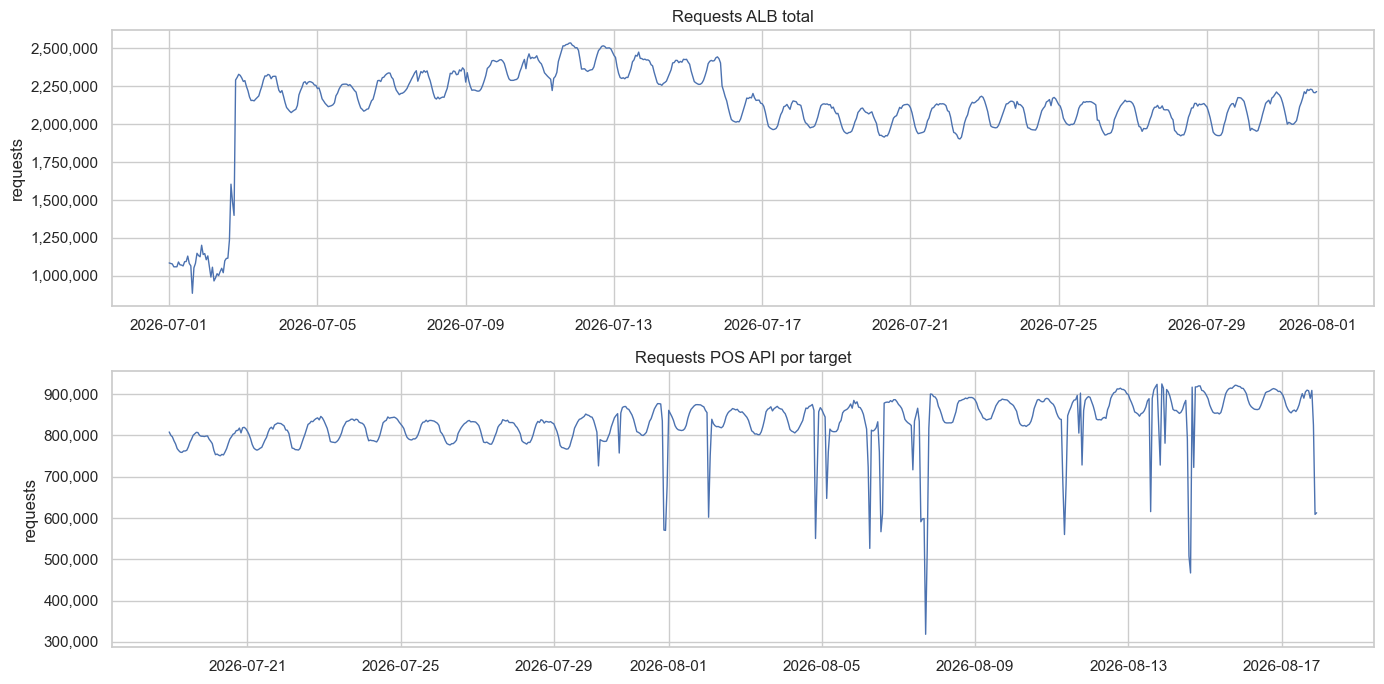
\includegraphics[width=\textwidth]{trafico_niveles.png}
\caption{Series de tráfico en niveles, con frecuencia horaria}
\label{fig:trafico_niveles}
\end{figure}

La naturaleza de esa oscilación se aprecia con mayor claridad en la
Figura~\ref{fig:perfil_horario}, que promedia el volumen para cada hora del día. Ambas series
describen un valle nocturno y un máximo vespertino. El balanceador alcanza su mínimo a las
07:00 y su máximo a las 21:00; la interfaz de punto de venta, su mínimo a las 08:00 y su
máximo a las 19:00. La amplitud del ciclo supera el diez por ciento del nivel medio, magnitud
que no admite tratarse como ruido.

\begin{figure}[htbp]
\centering
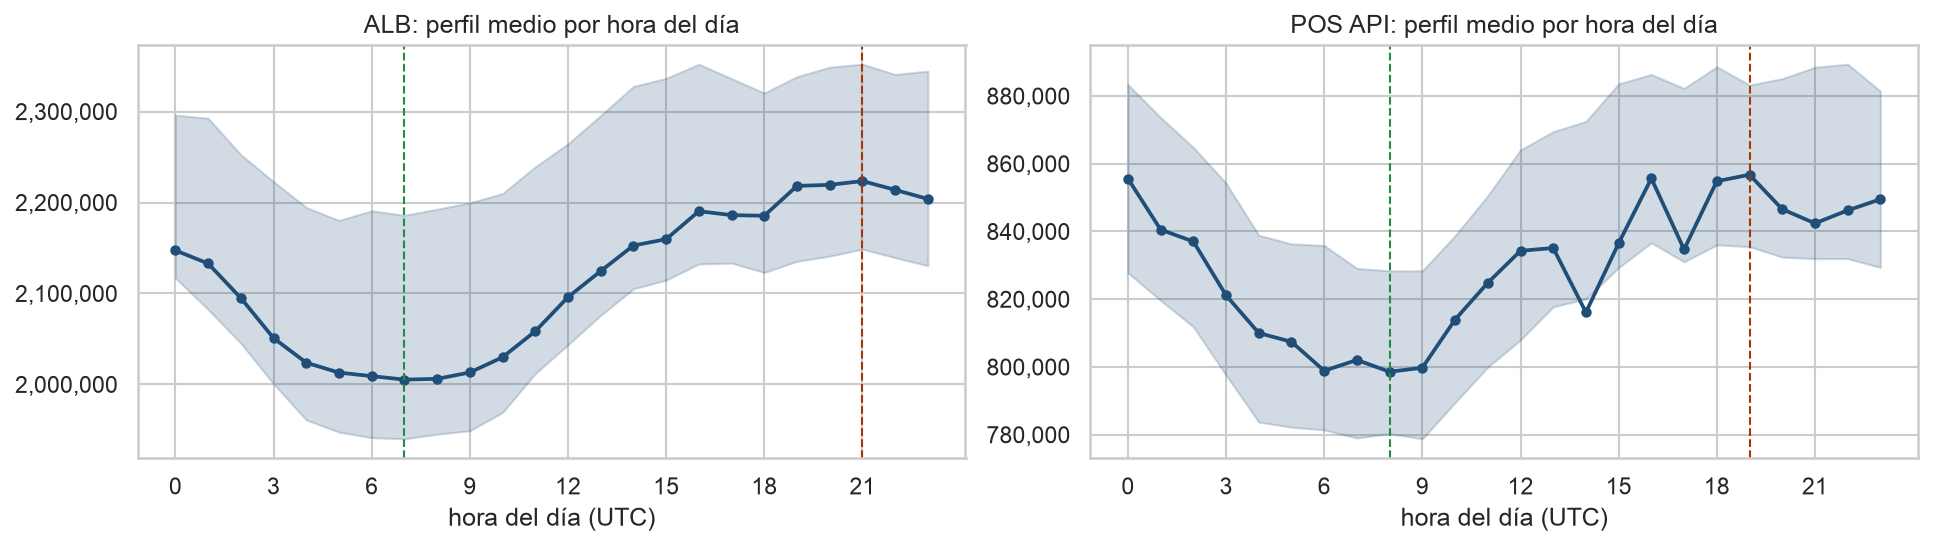
\includegraphics[width=\textwidth]{panel_perfil_horario.png}
\caption{Perfil medio por hora del día. La banda representa el rango intercuartílico; las líneas verticales señalan el máximo y el mínimo}
\label{fig:perfil_horario}
\end{figure}

La Figura~\ref{fig:heatmap} despliega la misma información sobre dos dimensiones y confirma la
regularidad del ciclo diario a lo largo de toda la semana.

\begin{figure}[htbp]
\centering
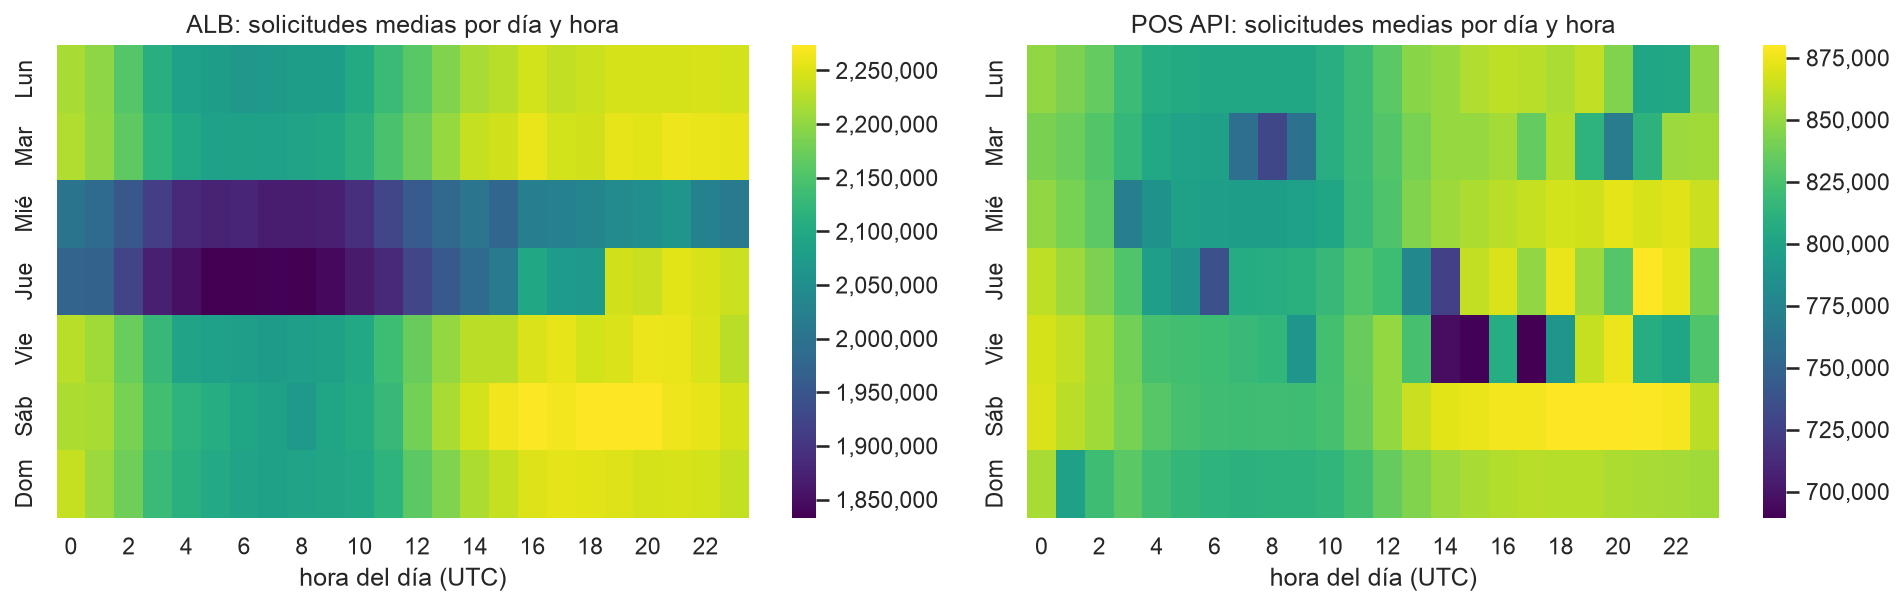
\includegraphics[width=\textwidth]{panel_heatmap.png}
\caption{Solicitudes medias según día de la semana y hora del día}
\label{fig:heatmap}
\end{figure}

Esta última figura revela además un rasgo que el trabajo no modela: en la serie del
balanceador, los días miércoles y jueves presentan niveles sensiblemente inferiores al resto
de la semana. Existe, por lo tanto, un efecto de día de la semana además del ciclo diario. El
período muestral de un mes ofrece apenas cuatro repeticiones de cada día, cantidad insuficiente
para estimar con fiabilidad una componente estacional de período 168. La limitación se retoma
en las conclusiones.

La Figura~\ref{fig:trafico_diferencias} compara el efecto de distintos esquemas de
diferenciación. La diferencia estacional de veinticuatro horas elimina el ciclo; la aplicación
adicional de una diferencia regular corrige el desplazamiento residual del nivel.

\begin{figure}[htbp]
\centering
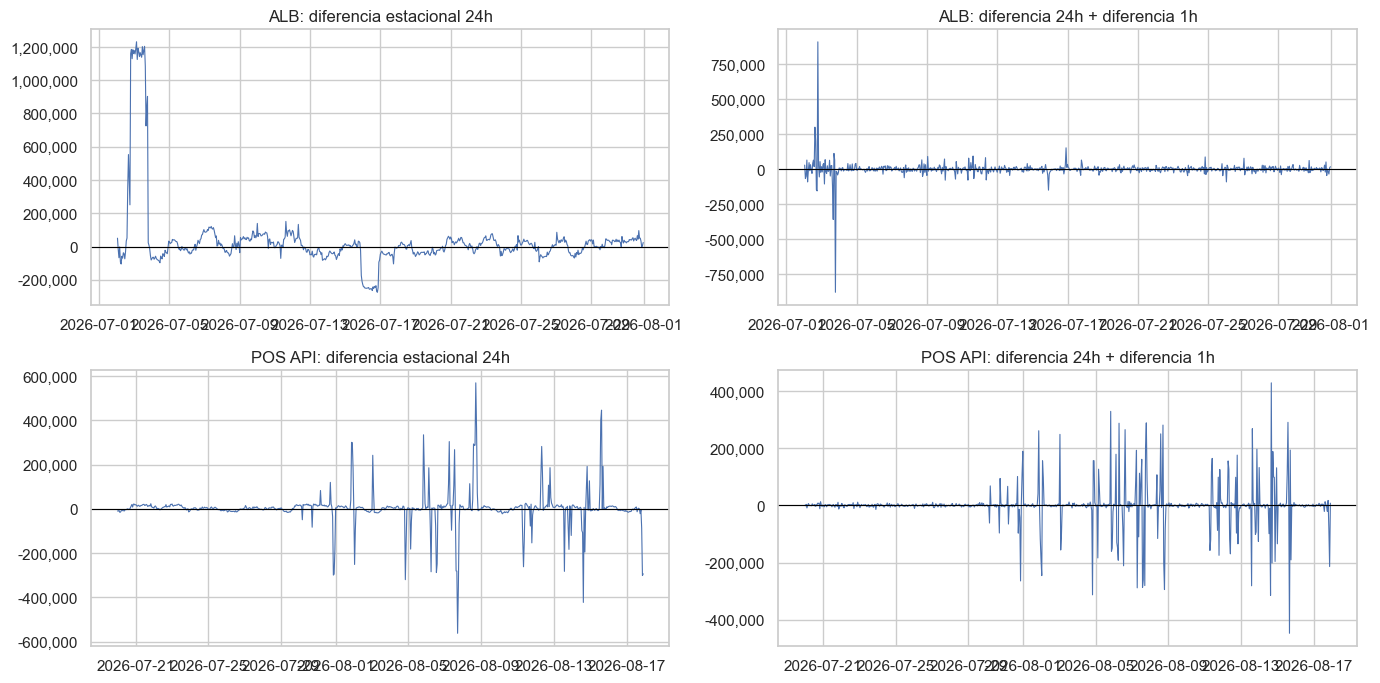
\includegraphics[width=\textwidth]{trafico_diferencias.png}
\caption{Efecto de la diferencia estacional y de su combinación con la diferencia regular}
\label{fig:trafico_diferencias}
\end{figure}

\subsubsection{Serie de altitud}

La Figura~\ref{fig:uav_niveles} presenta la serie de altitud en niveles y su primera
diferencia. El comportamiento difiere por completo del anterior: no hay ciclo repetitivo sino
un recorrido con fases sucesivas de despegue, ascenso, crucero y descenso. La media se desplaza sin retorno, señal visual de no estacionariedad. La primera
diferencia oscila en torno a cero con dispersión estable.

\begin{figure}[htbp]
\centering
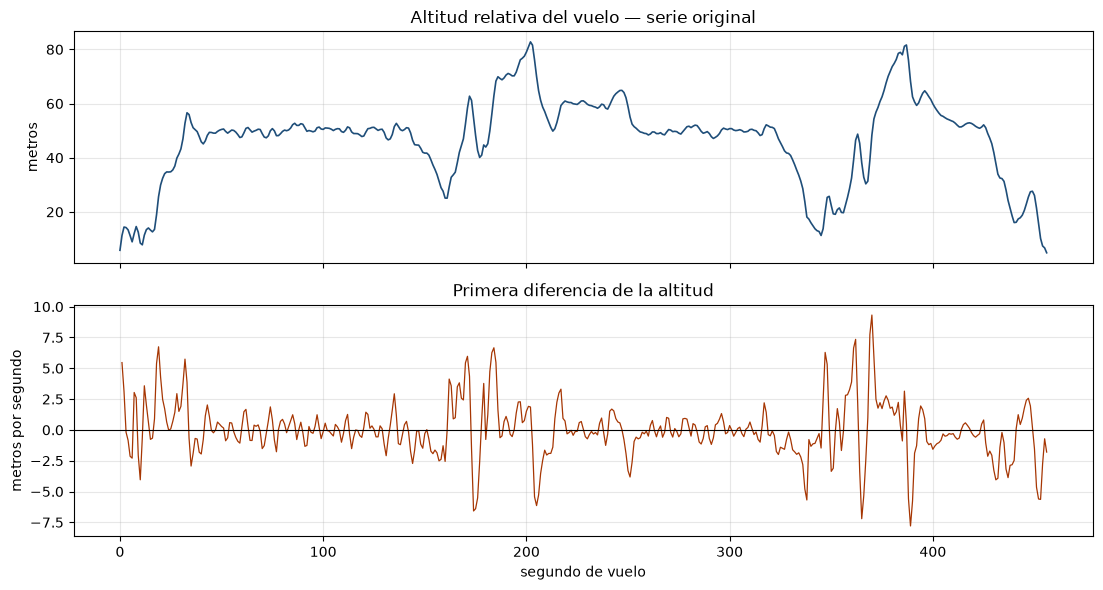
\includegraphics[width=\textwidth]{uav_niveles_diff.png}
\caption{Altitud relativa del vuelo en niveles y en primera diferencia}
\label{fig:uav_niveles}
\end{figure}

\subsection{Funciones de autocovarianza, autocorrelación y autocorrelación parcial (punto 3)}

La Figura~\ref{fig:trafico_facs} presenta las tres funciones para las series de tráfico. El
rasgo determinante son los picos pronunciados en los rezagos 24, 48 y 72, que confirman la
periodicidad diaria y fijan el período estacional en $s = 24$. La autocorrelación no decae
hacia cero entre esos picos, lo cual indica que la componente estacional domina la estructura.
La Figura~\ref{fig:pos_facs} reproduce el mismo conjunto para la serie de punto de venta, con
un patrón equivalente.

\begin{figure}[htbp]
\centering
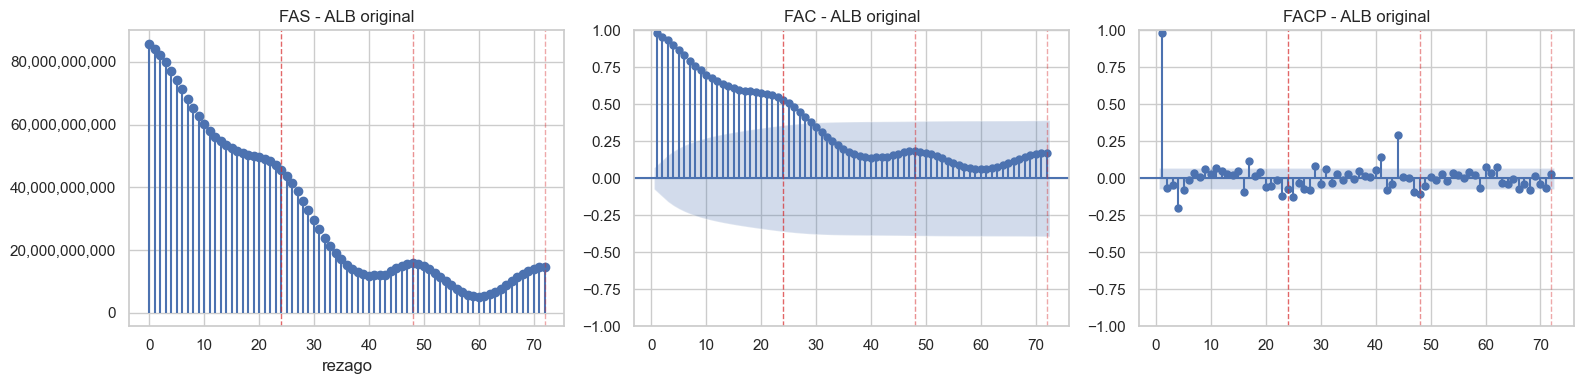
\includegraphics[width=\textwidth]{trafico_fasfacfacp_1.png}
\caption{Funciones FAS, FAC y FACP de la serie del balanceador de carga}
\label{fig:trafico_facs}
\end{figure}

\begin{figure}[htbp]
\centering
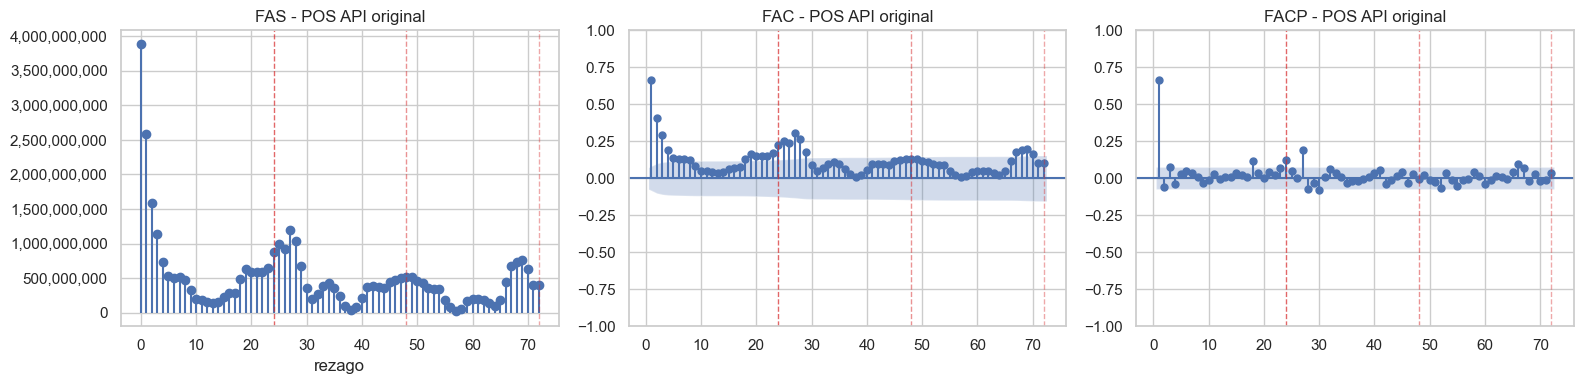
\includegraphics[width=\textwidth]{trafico_fasfacfacp_2.png}
\caption{Funciones FAS, FAC y FACP de la serie de punto de venta}
\label{fig:pos_facs}
\end{figure}

La Figura~\ref{fig:uav_facs} presenta el mismo conjunto para la serie de altitud, en niveles y
tras diferenciar. El contraste ilustra el concepto expuesto en el marco teórico con más claridad que cualquier descripción. En niveles, la autocorrelación de primer orden alcanza 0,96 y decae con
lentitud casi lineal, mientras la parcial exhibe un primer rezago cercano a la unidad y se
corta de inmediato. La teoría asocia ese par de patrones a un proceso integrado: la
persistencia no proviene de una memoria autorregresiva de orden elevado sino de la presencia de
una raíz unitaria, y el remedio es la diferenciación.

\begin{figure}[htbp]
\centering
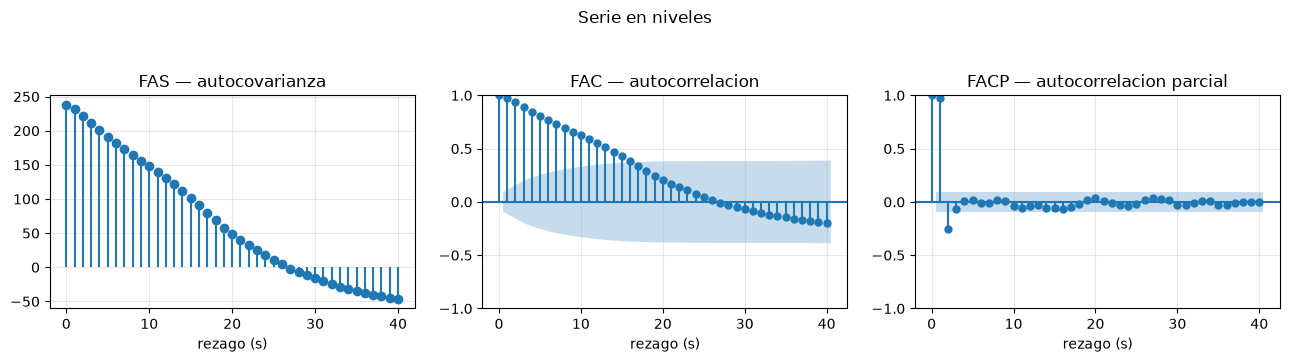
\includegraphics[width=0.92\textwidth]{uav_fasfacfacp_1.png}
\caption{Funciones FAS, FAC y FACP de la altitud en niveles}
\label{fig:uav_facs}
\end{figure}

\begin{figure}[htbp]
\centering
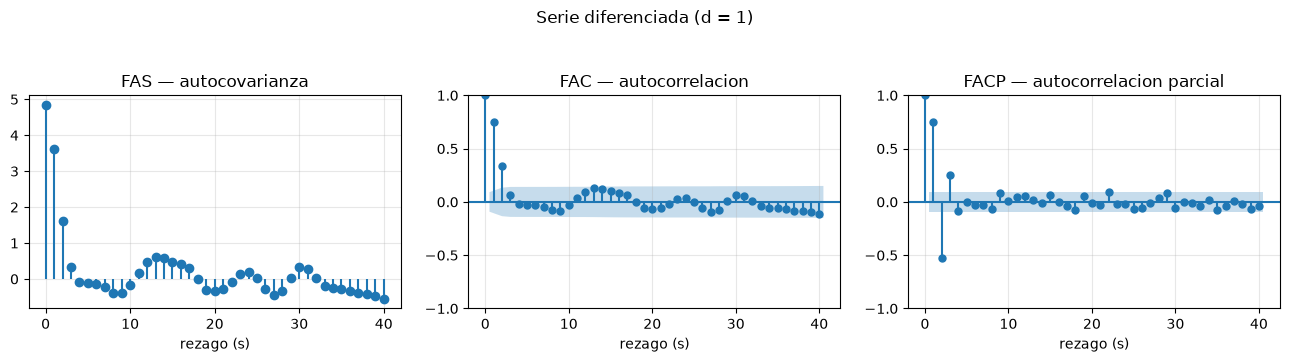
\includegraphics[width=0.92\textwidth]{uav_fasfacfacp_2.png}
\caption{Funciones FAS, FAC y FACP de la altitud tras una diferencia regular}
\label{fig:uav_facs_diff}
\end{figure}

Tras la diferenciación, la autocorrelación pierde la persistencia y conserva significatividad
únicamente en los primeros rezagos, patrón compatible con una componente de medias móviles de orden bajo. El material identificado, visible en la Figura~\ref{fig:uav_facs_diff}, corresponde a un
modelo ARIMA$(p,1,q)$ con órdenes reducidos.

\subsection{Pruebas de raíces unitarias (punto 4)}

La Tabla~\ref{tab:raices} reúne los resultados de ambos contrastes sobre las series de tráfico
en sus distintas versiones.

\begin{table}[htbp]
\centering
\caption{Contrastes de raíces unitarias sobre las series de tráfico}
\label{tab:raices}
\small
\begin{tabular}{llrrrr}
\toprule
\textbf{Serie} & \textbf{Versión} & \textbf{ADF} & \textbf{$p$} & \textbf{KPSS} & \textbf{$p$} \\
\midrule
Balanceador & original & $-4{,}53$ & 0,00 & 0,41 & 0,07 \\
Balanceador & difer. regular & $-9{,}70$ & 0,00 & 0,17 & 0,10 \\
Balanceador & difer. estacional & $-7{,}56$ & 0,00 & 0,54 & 0,03 \\
Balanceador & ambas diferencias & $-10{,}10$ & 0,00 & 0,02 & 0,10 \\
\addlinespace
Punto de venta & original & $-9{,}55$ & 0,00 & 2,33 & 0,01 \\
Punto de venta & difer. regular & $-10{,}82$ & 0,00 & 0,13 & 0,10 \\
Punto de venta & difer. estacional & $-6{,}21$ & 0,00 & 0,02 & 0,10 \\
Punto de venta & ambas diferencias & $-10{,}43$ & 0,00 & 0,24 & 0,10 \\
\bottomrule
\end{tabular}
\end{table}

La lectura conjunta revela un matiz que un contraste aislado ocultaría. Sobre la serie del
balanceador en niveles, ambas pruebas coinciden en la estacionariedad. Sobre la serie de punto
de venta en niveles, en cambio, discrepan: la prueba de Dickey-Fuller aumentada rechaza la
raíz unitaria, pero la KPSS rechaza también la estacionariedad. Esa configuración es típica de series con componente estacional marcada, donde cada contraste interpreta la estructura periódica de un modo distinto.

El caso de la serie de altitud aporta un tercer escenario. La prueba de Dickey-Fuller aumentada
arroja $p = 0{,}1237$ y no rechaza la raíz unitaria; la KPSS arroja $p \geq 0{,}10$ y tampoco
rechaza la estacionariedad. Ninguna de las dos se pronuncia.

Ante esa indefinición, la decisión de diferenciar se sostiene sobre tres elementos
convergentes: el desplazamiento visible de la media, el decaimiento lento de la autocorrelación
junto con el corte abrupto de la parcial, y la ausencia de rechazo por parte de la prueba de
Dickey-Fuller aumentada. La literatura recomienda diferenciar ante evidencia de raíz unitaria,
porque sobrediferenciar cuesta menos que estimar sobre una serie integrada \parencite{hyndman2021}.

El resultado decisivo aparece tras la diferenciación. La prueba de Ljung-Box aplicada a la
serie de altitud diferenciada arroja $p = 1{,}115 \times 10^{-62}$ y rechaza la incorrelación sin margen de duda. Subsiste, por lo tanto, estructura autocorrelacionada genuina, y
existe un modelo por estimar.

\begin{lstlisting}[caption={Aplicación conjunta de ambos contrastes}]
p_adf = adfuller(datos)[1]            # H0: existe raiz unitaria
p_kpss = kpss(datos, nlags="auto")[1] # H0: la serie es estacionaria
\end{lstlisting}

\subsection{Estimación y selección de modelos (punto 5)}

\subsubsection{Series de tráfico}

Se estimó una grilla de modelos SARIMA con período estacional $s = 24$, con distintas
combinaciones de diferencia regular y estacional. La Tabla~\ref{tab:sarima} presenta los ocho
modelos resultantes.

La comparación emplea dos criterios complementarios. Los criterios de información miden el
ajuste dentro de la muestra y penalizan la cantidad de parámetros; el desempeño sobre el
conjunto de prueba evalúa la capacidad predictiva efectiva. Cuando ambos coinciden, la elección es inmediata; cuando discrepan, se privilegia el desempeño fuera de muestra, que atiende directamente a la finalidad predictiva del modelo.

\begin{table}[htbp]
\centering
\caption{Comparación de modelos SARIMA estimados}
\label{tab:sarima}
\small
\begin{tabular}{llrrrr}
\toprule
\textbf{Serie} & \textbf{Modelo} & \textbf{AIC} & \textbf{BIC} & \textbf{MAE} & \textbf{MAPE} \\
\midrule
Balanceador & $\mathbf{(1,1,1)\times(1,1,1)_{24}}$ & \textbf{15.491,11} & 15.513,46 & \textbf{16.662} & \textbf{0,79\,\%} \\
Balanceador & $(1,0,1)\times(1,1,1)_{24}$ & 15.527,20 & 15.549,55 & 26.776 & 1,26\,\% \\
Balanceador & $(1,1,1)\times(1,0,1)_{24}$ & 16.229,29 & 16.251,82 & 76.284 & 3,74\,\% \\
Balanceador & $(1,0,1)\times(1,0,1)_{24}$ & 16.264,80 & 16.287,34 & 74.059 & 3,64\,\% \\
\addlinespace
Punto de venta & $(1,0,1)\times(1,1,1)_{24}$ & \textit{15.381,30} & 15.403,47 & 39.594 & 5,09\,\% \\
Punto de venta & $(1,1,1)\times(1,1,1)_{24}$ & 15.467,63 & 15.489,79 & 45.861 & 5,91\,\% \\
Punto de venta & $\mathbf{(1,1,1)\times(1,0,1)_{24}}$ & 15.737,10 & 15.759,45 & \textbf{29.641} & \textbf{3,90\,\%} \\
Punto de venta & $(1,0,1)\times(1,0,1)_{24}$ & 15.860,56 & 15.882,91 & 30.840 & 4,08\,\% \\
\bottomrule
\end{tabular}


\vspace{0.4em}
{\footnotesize\textit{Nota.} En negrita, el modelo seleccionado para cada serie. En cursiva, el
valor mínimo del criterio de Akaike cuando no corresponde al modelo seleccionado.\par}
\end{table}

En la serie del balanceador ambos criterios coinciden: la especificación
$(1,1,1)\times(1,1,1)_{24}$ minimiza simultáneamente el criterio de Akaike y el error de
predicción.

En la serie de punto de venta, en cambio, \textbf{los criterios discrepan}. El de Akaike favorece la
especificación $(1,0,1)\times(1,1,1)_{24}$, con un valor de 15.381,30; el desempeño sobre el
conjunto de prueba favorece $(1,1,1)\times(1,0,1)_{24}$, cuyo error porcentual absoluto medio cae casi un tercio, 3,90 frente a 5,09 por ciento.

Se adopta esta última. La discrepancia admite una lectura sustantiva: la diferencia estacional
mejora el ajuste dentro de la muestra pero deteriora la predicción, comportamiento característico
de una componente estacional menos estable que en la serie del balanceador. El criterio empleado
es el mismo que se aplica más adelante al seleccionar el orden del modelo multivariado, donde la
divergencia entre criterios se manifiesta con mayor intensidad.

El examen de significatividad individual deja un resultado incómodo, que este informe prefiere
exponer antes que atenuar. En el modelo del balanceador, los parámetros de la parte regular carecen de
significatividad: el coeficiente autorregresivo alcanza $-0{,}08$ con $p = 0{,}97$, y el de
medias móviles $0{,}01$ con $p = 1{,}00$. Los parámetros estacionales, en cambio, son
altamente significativos: $-0{,}15$ con $p < 0{,}001$ para el autorregresivo y $-0{,}52$ con
$p < 0{,}001$ para el de medias móviles.

La lectura es que la estructura de la serie reside casi por completo en su componente
estacional, y la parte regular del modelo sobra. Una especificación
$(0,1,0)\times(1,1,1)_{24}$ habría alcanzado un ajuste equivalente con dos parámetros menos.

\subsubsection{Serie de altitud}

Sobre la serie de altitud se estimó una grilla ARIMA$(p,1,q)$ con órdenes entre cero y tres.
El criterio de Akaike selecciona ARIMA$(1,1,3)$, con un valor de 1.379,95.

\begin{lstlisting}[caption={Grilla de modelos y selección por criterio de información}]
for p in range(4):
    for q in range(4):
        ajuste = ARIMA(entrenamiento, order=(p, 1, q)).fit()
        resultados.append({"modelo": f"ARIMA({p},1,{q})", "AIC": ajuste.aic})
\end{lstlisting}

A diferencia del caso anterior, los cuatro parámetros son individualmente significativos al cinco
por ciento, según se detalla en la Tabla~\ref{tab:uav_params}.

\begin{table}[htbp]
\centering
\caption{Parámetros del modelo ARIMA$(1,1,3)$ de la serie de altitud}
\label{tab:uav_params}
\small
\begin{tabular}{lrrrr}
\toprule
\textbf{Parámetro} & \textbf{Coeficiente} & \textbf{Error estándar} & \textbf{$z$} & \textbf{$P>|z|$} \\
\midrule
$\phi_1$ & $-0{,}2650$ & 0,120 & $-2{,}208$ & 0,027 \\
$\theta_1$ & 1,6263 & 0,113 & 14,432 & $<0{,}001$ \\
$\theta_2$ & 1,2023 & 0,136 & 8,821 & $<0{,}001$ \\
$\theta_3$ & 0,4268 & 0,061 & 6,959 & $<0{,}001$ \\
$\sigma^2$ & 1,3022 & 0,051 & 25,344 & $<0{,}001$ \\
\bottomrule
\end{tabular}
\end{table}

La significatividad conjunta se evaluó mediante el contraste de razón de verosimilitud contra
el modelo restringido ARIMA$(0,1,0)$, equivalente a un paseo aleatorio sin parámetros. El
estadístico alcanza 567,11 con cuatro grados de libertad y un valor $p$ del orden de
$2 \times 10^{-121}$. La hipótesis nula de nulidad conjunta se rechaza sin margen de duda.

\begin{lstlisting}[caption={Contraste de significatividad global por razón de verosimilitud}]
modelo_nulo = ARIMA(entrenamiento, order=(0, 1, 0)).fit()
estadistico_lr = 2 * (modelo.llf - modelo_nulo.llf)
p_valor = stats.chi2.sf(estadistico_lr, len(modelo.params) - len(modelo_nulo.params))
\end{lstlisting}

\subsection{Desempeño y comparación entre modelos (puntos 6 y 7)}

La partición entre entrenamiento y prueba reservó las últimas 48 horas en las series de
tráfico y los últimos 15 segundos en la de altitud. Ambos horizontes guardan proporción con la
frecuencia de muestreo y con el tamaño de la muestra. La Tabla~\ref{tab:metricas} reúne el
desempeño de los modelos seleccionados.

\begin{table}[htbp]
\centering
\caption{Desempeño de los modelos seleccionados sobre el conjunto de prueba}
\label{tab:metricas}
\small
\begin{tabular}{llrrr}
\toprule
\textbf{Serie} & \textbf{Modelo} & \textbf{MAE} & \textbf{RMSE} & \textbf{MAPE} \\
\midrule
Balanceador & SARIMA$(1,1,1)\times(1,1,1)_{24}$ & 16.662 & 20.310 & 0,79\,\% \\
Punto de venta & SARIMA$(1,1,1)\times(1,0,1)_{24}$ & 29.641 & 58.454 & 3,90\,\% \\
Altitud (m) & ARIMA$(1,1,3)$ & 6,01 & 7,53 & --- \\
\bottomrule
\end{tabular}
\end{table}

La comparación entre modelos, presentada en la Tabla~\ref{tab:sarima}, muestra cuánto separa a las especificaciones con diferencia estacional de las que carecen de ella. En la serie del balanceador, el error absoluto medio se multiplica por cuatro al
omitirla. La componente estacional es, pues, el elemento decisivo.

En el caso de la serie de altitud, las diferencias entre órdenes vecinos son mínimas: los
cuatro mejores modelos por criterio de Akaike presentan errores absolutos medios comprendidos
entre 5,99 y 6,01 metros. El desempeño predictivo no discrimina, y el criterio de información
opera como desempate en favor de la especificación más parsimoniosa.

Corresponde advertir que el conjunto de prueba de la serie de altitud coincide con la fase de
descenso, dinámicamente distinta del crucero donde el modelo se entrena en su mayor parte. La métrica obtenida peca, pues, de conservadora.

\subsection{Diagnóstico de residuos (punto 8)}

El diagnóstico arroja resultados netamente distintos entre las series de tráfico y la de
altitud, y conviene exponerlos por separado.

\subsubsection{Series de tráfico}

La Tabla~\ref{tab:ljung_trafico} presenta la prueba de Ljung-Box sobre los residuos de ambos
modelos.

\begin{table}[htbp]
\centering
\caption{Prueba de Ljung-Box sobre los residuos de los modelos SARIMA}
\label{tab:ljung_trafico}
\small
\begin{tabular}{lrrl}
\toprule
\textbf{Serie} & \textbf{Rezago} & \textbf{Estadístico} & \textbf{$p$} \\
\midrule
Balanceador & 12 & 17,40 & 0,14 \\
Balanceador & 24 & 43,64 & 0,01 \\
Balanceador & 48 & 212,49 & $<0{,}001$ \\
\addlinespace
Punto de venta & 12 & 86,58 & $<0{,}001$ \\
Punto de venta & 24 & 92,07 & $<0{,}001$ \\
Punto de venta & 48 & 112,38 & $<0{,}001$ \\
\bottomrule
\end{tabular}
\end{table}

El resultado es desfavorable y así debe consignarse. En la serie del balanceador, los
residuos superan el contraste hasta el rezago 12, pero lo incumplen a partir del rezago 24. En
la serie de punto de venta, el rechazo se verifica en todos los rezagos examinados.

La implicación es que ambos modelos dejan estructura sin explicar, concentrada en los rezagos
correspondientes al ciclo diario y a sus múltiplos. El patrón concuerda con lo observado en el mapa de calor: existe una componente semanal que los
modelos no capturan, y que se manifiesta como autocorrelación residual en los rezagos
estacionales.

Las Figuras~\ref{fig:res_alb} y~\ref{fig:res_pos} muestran ese comportamiento: la función de
autocorrelación de los residuos conserva coeficientes significativos en los rezagos múltiplos
de veinticuatro.

En consecuencia, los pronósticos de estas dos series deben interpretarse con menor confianza
que la sugerida por sus métricas de error, y los intervalos de predicción son probablemente demasiado estrechos.

\begin{figure}[htbp]
\centering
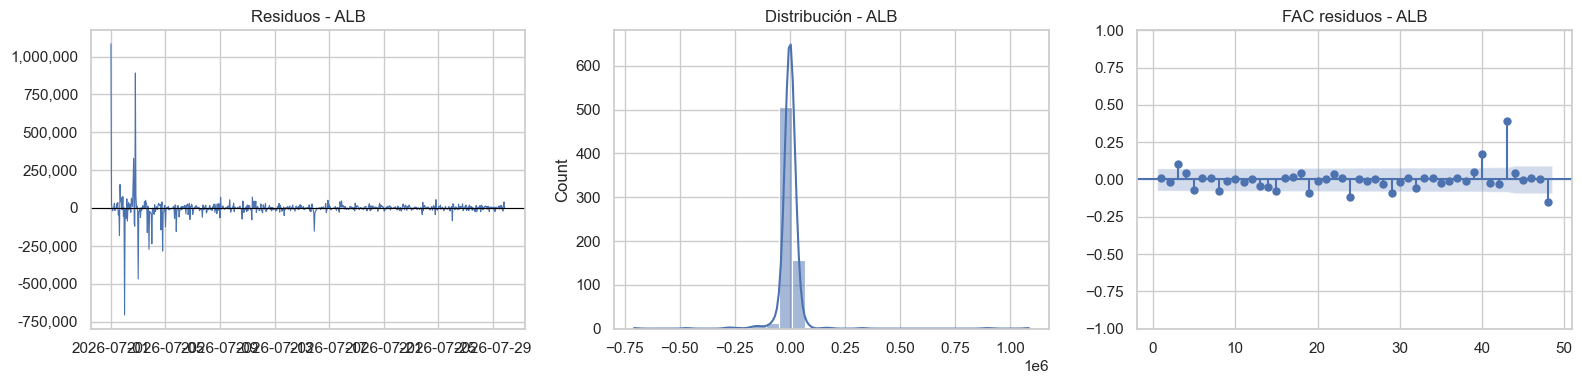
\includegraphics[width=\textwidth]{trafico_residuos_1.png}
\caption{Diagnóstico de residuos del modelo de la serie del balanceador de carga}
\label{fig:res_alb}
\end{figure}

\begin{figure}[htbp]
\centering
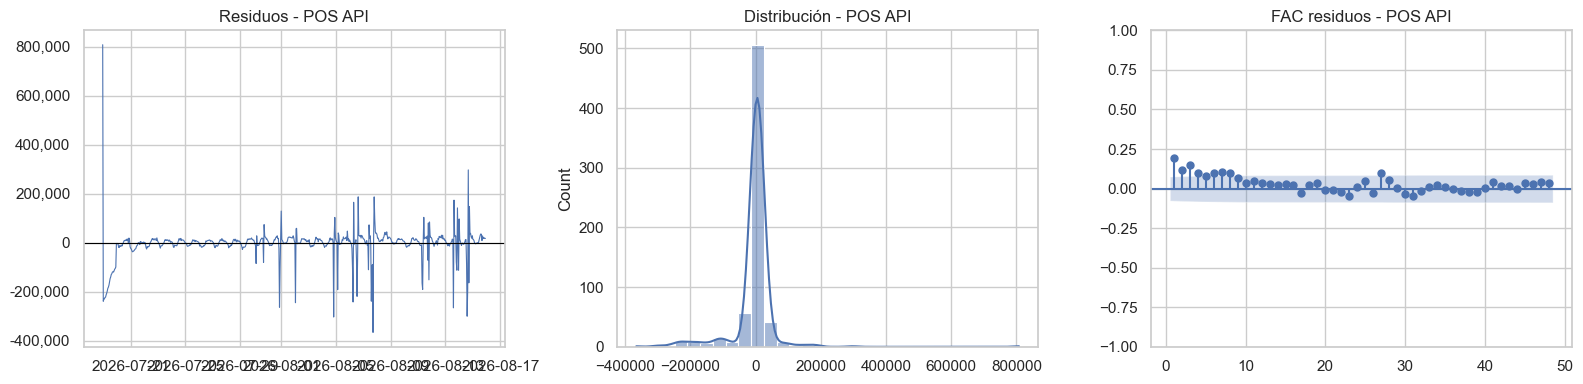
\includegraphics[width=\textwidth]{trafico_residuos_2.png}
\caption{Diagnóstico de residuos del modelo de la serie de punto de venta}
\label{fig:res_pos}
\end{figure}

\subsubsection{Serie de altitud}

El diagnóstico del modelo ARIMA$(1,1,3)$ arroja el resultado opuesto. La prueba de Ljung-Box no
rechaza la incorrelación en ninguno de los rezagos examinados: $p = 0{,}976$ en el rezago 10,
$p = 0{,}631$ en el 20 y $p = 0{,}487$ en el 30. Los residuos tienen media de 0,0136 metros y desvío estándar de 1,1644 metros.

\begin{figure}[htbp]
\centering
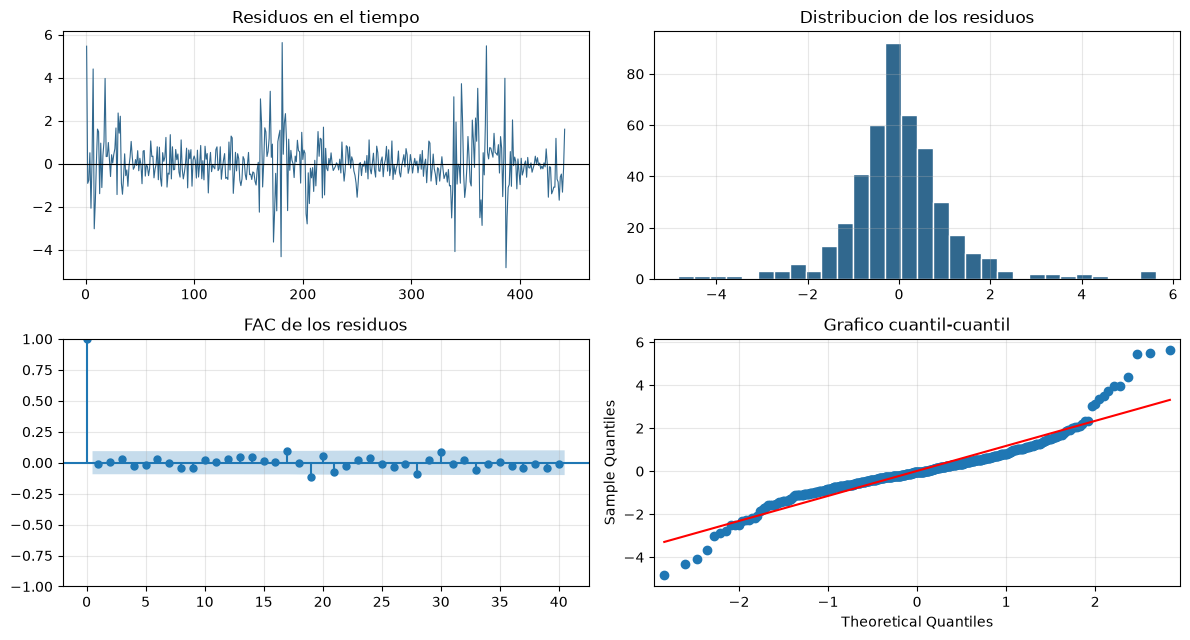
\includegraphics[width=\textwidth]{uav_residuos.png}
\caption{Diagnóstico de residuos del modelo de la serie de altitud}
\label{fig:res_uav}
\end{figure}

La Figura~\ref{fig:res_uav} confirma el resultado: los coeficientes de la función de
autocorrelación de los residuos permanecen dentro de la banda de significatividad, y el
gráfico temporal no evidencia cambios sistemáticos de nivel ni de dispersión.

El modelo no deja estructura autocorrelacionada sin explicar. El contraste de Jarque-Bera \parencite{jarque1980}, en
cambio, rechaza la normalidad con un estadístico de 431,74, asimetría de 0,51 y curtosis de
7,74. Los apartamientos se concentran en las colas y se explican por las maniobras del vuelo; afectan la validez de los intervalos de confianza nominales, no la estimación puntual.

\subsection{Pronósticos (punto 9)}

La Figura~\ref{fig:pron_trafico} presenta los pronósticos a 48 horas de las series de tráfico.
El horizonte equivale a dos ciclos diarios completos, ventana que permite verificar si el
modelo reproduce la periodicidad sin extrapolar en exceso. La Figura~\ref{fig:pron_pos}
presenta el correspondiente a la serie de punto de venta.

\begin{figure}[htbp]
\centering
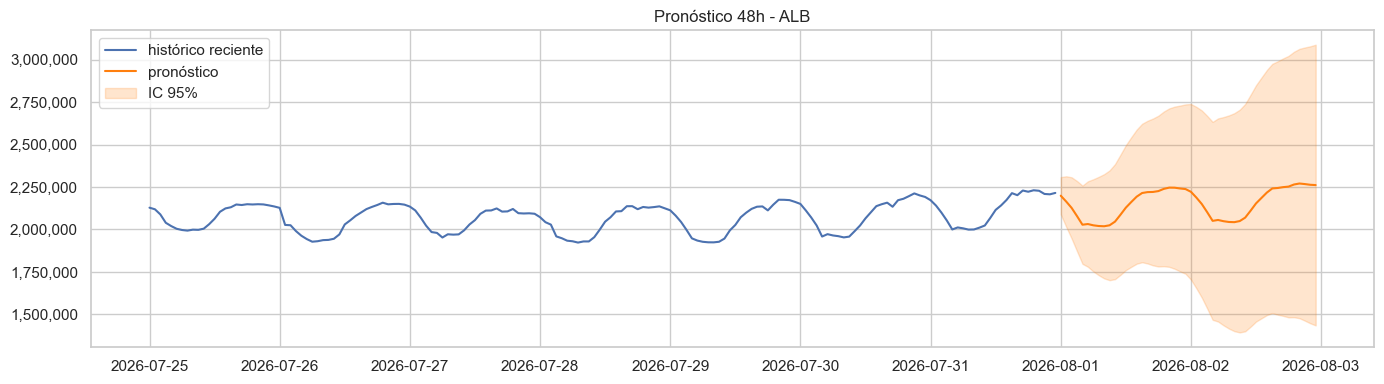
\includegraphics[width=\textwidth]{trafico_pronostico_1.png}
\caption{Pronóstico a 48 horas de la serie del balanceador de carga}
\label{fig:pron_trafico}
\end{figure}

\begin{figure}[htbp]
\centering
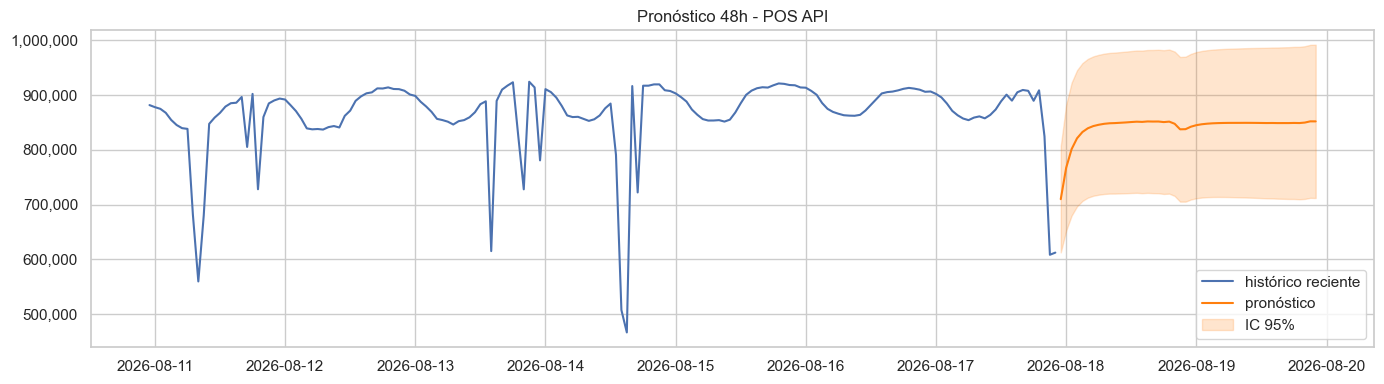
\includegraphics[width=\textwidth]{trafico_pronostico_2.png}
\caption{Pronóstico a 48 horas de la serie de punto de venta}
\label{fig:pron_pos}
\end{figure}

La Figura~\ref{fig:pron_uav} presenta el pronóstico a 15 segundos de la serie de altitud. El
horizonte responde a la frecuencia de un hertz y al tamaño de la muestra, y representa poco más
del tres por ciento de las observaciones. Un horizonte de 45 segundos eleva el error absoluto
medio por encima de los 18 metros, dado que abarca la maniobra de descenso completa.

\begin{figure}[htbp]
\centering
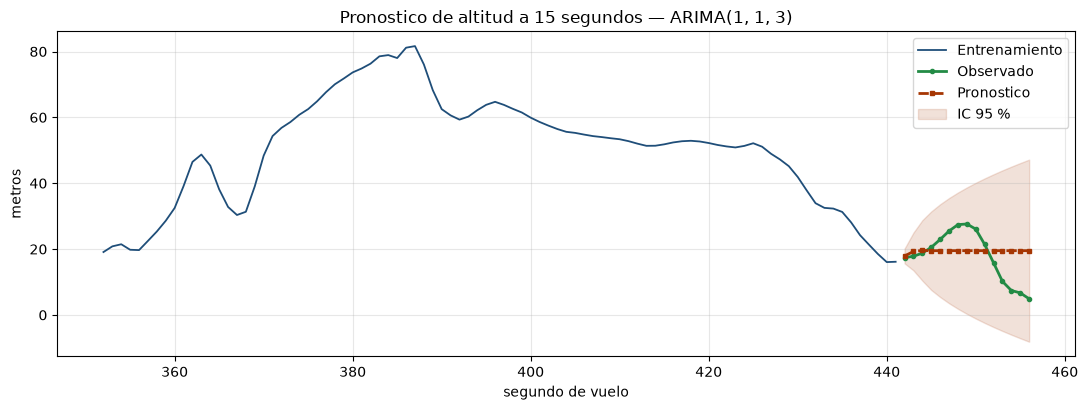
\includegraphics[width=\textwidth]{uav_pronostico.png}
\caption{Pronóstico a 15 segundos de la serie de altitud, con intervalo de confianza}
\label{fig:pron_uav}
\end{figure}

\subsection{Modelo de vectores autorregresivos (punto 10)}

\subsubsection{Alcance y restricción de calendario}

El modelo multivariado se construye sobre las dos series de tráfico. La serie de altitud queda
excluida por una razón que no admite solución dentro del conjunto de datos disponible: fue
registrada en 2018, mientras que las series de tráfico corresponden a 2026. Los calendarios son
disjuntos y no comparten un solo instante de observación. Un modelo de vectores autorregresivos
exige series alineadas sobre el mismo eje temporal, de modo que construirlo con las tres es técnicamente imposible.

Las dos series de tráfico tampoco coinciden por completo. La intersección temporal abarca desde
el 18 de julio hasta el 31 de julio de 2026, esto es, trece días. Tras aplicar la
transformación logarítmica y la diferencia estacional restan 289 observaciones.

\begin{lstlisting}[caption={Alineación temporal y transformación previa al modelo multivariado}]
alineadas = pd.concat([alb, pos], axis=1, join="inner").dropna()
datos_var = np.log1p(alineadas).diff(24).dropna()
\end{lstlisting}

\subsubsection{Selección del orden de rezagos}

Los cuatro criterios de selección no coinciden, según muestra la Tabla~\ref{tab:var_orden}.

\begin{table}[htbp]
\centering
\caption{Orden de rezagos sugerido por cada criterio}
\label{tab:var_orden}
\small
\begin{tabular}{lr}
\toprule
\textbf{Criterio} & \textbf{Rezagos} \\
\midrule
Akaike & 24 \\
Bayesiano & 2 \\
Hannan-Quinn & 2 \\
Error de predicción final & 24 \\
\bottomrule
\end{tabular}
\end{table}

La discrepancia tiene consecuencias considerables. Con dos variables y 24 rezagos, el modelo
estima 98 parámetros a partir de 241 observaciones de entrenamiento, relación que compromete la
fiabilidad de las estimaciones. Con dos rezagos, el número desciende a 10.

El desempeño fuera de muestra resuelve el empate. La Tabla~\ref{tab:var_comp} compara
especificaciones alternativas mediante métricas calculadas sobre la escala original.

\begin{table}[htbp]
\centering
\caption{Comparación de especificaciones del modelo multivariado a 48 horas}
\label{tab:var_comp}
\small
\begin{tabular}{rrrrrr}
\toprule
\textbf{Rezagos} & \textbf{Parám.} & \textbf{MAE bal.} & \textbf{MAPE bal.} & \textbf{MAE p.\ venta} & \textbf{MAPE p.\ venta} \\
\midrule
1 & 6 & 31.287 & 1,48\,\% & 32.128 & 4,67\,\% \\
\textbf{2} & \textbf{10} & \textbf{27.826} & \textbf{1,31\,\%} & \textbf{31.455} & \textbf{4,59\,\%} \\
3 & 14 & 26.275 & 1,24\,\% & 30.781 & 4,51\,\% \\
24 & 98 & 36.008 & 1,71\,\% & 26.932 & 4,03\,\% \\
\bottomrule
\end{tabular}
\end{table}

El resultado es un caso de manual de sobreajuste. La especificación con 24 rezagos, pese
a emplear casi diez veces más parámetros, predice \textit{peor} la serie del balanceador que la
de dos rezagos. Su única ventaja aparece en la serie de punto de venta, donde reduce el error absoluto
medio un catorce por ciento, mejora que no compensa multiplicar por diez el número de parámetros.

Se adopta entonces la especificación con \textbf{dos rezagos}, respaldada por dos
criterios de información y por el desempeño fuera de muestra. La alternativa de tres rezagos
mejora levemente ambas métricas, pero ningún criterio de información la respalda.

\subsubsection{Sobre la medición del error}

Las métricas de la Tabla~\ref{tab:var_comp} se calculan sobre la escala original, en
solicitudes, tras invertir la transformación aplicada. La precisión no es accesoria. Calculadas
sobre la serie transformada, que oscila en torno a cero, las mismas predicciones arrojaban un
error porcentual absoluto medio del 97,20 por ciento, cifra que sugería un modelo inservible.

El valor no reflejaba la calidad del modelo sino la inadecuación de la métrica: al dividir por
un denominador próximo a cero, el error porcentual se vuelve inestable y carece de
interpretación \parencite{hyndman2006}. Expresado en la escala original, el mismo modelo
alcanza un error del 1,31 por ciento.

\begin{lstlisting}[caption={Inversión de la transformación previa al cálculo de métricas}]
for i, t in enumerate(indice_prueba):
    base = historico.loc[t - pd.Timedelta(hours=24)]
    historico.loc[t] = base + pronostico_transformado.iloc[i]
prediccion = np.expm1(historico.reindex(indice_prueba).to_numpy())
\end{lstlisting}

La Figura~\ref{fig:var_pron} presenta el pronóstico resultante sobre la escala original.

\begin{figure}[htbp]
\centering
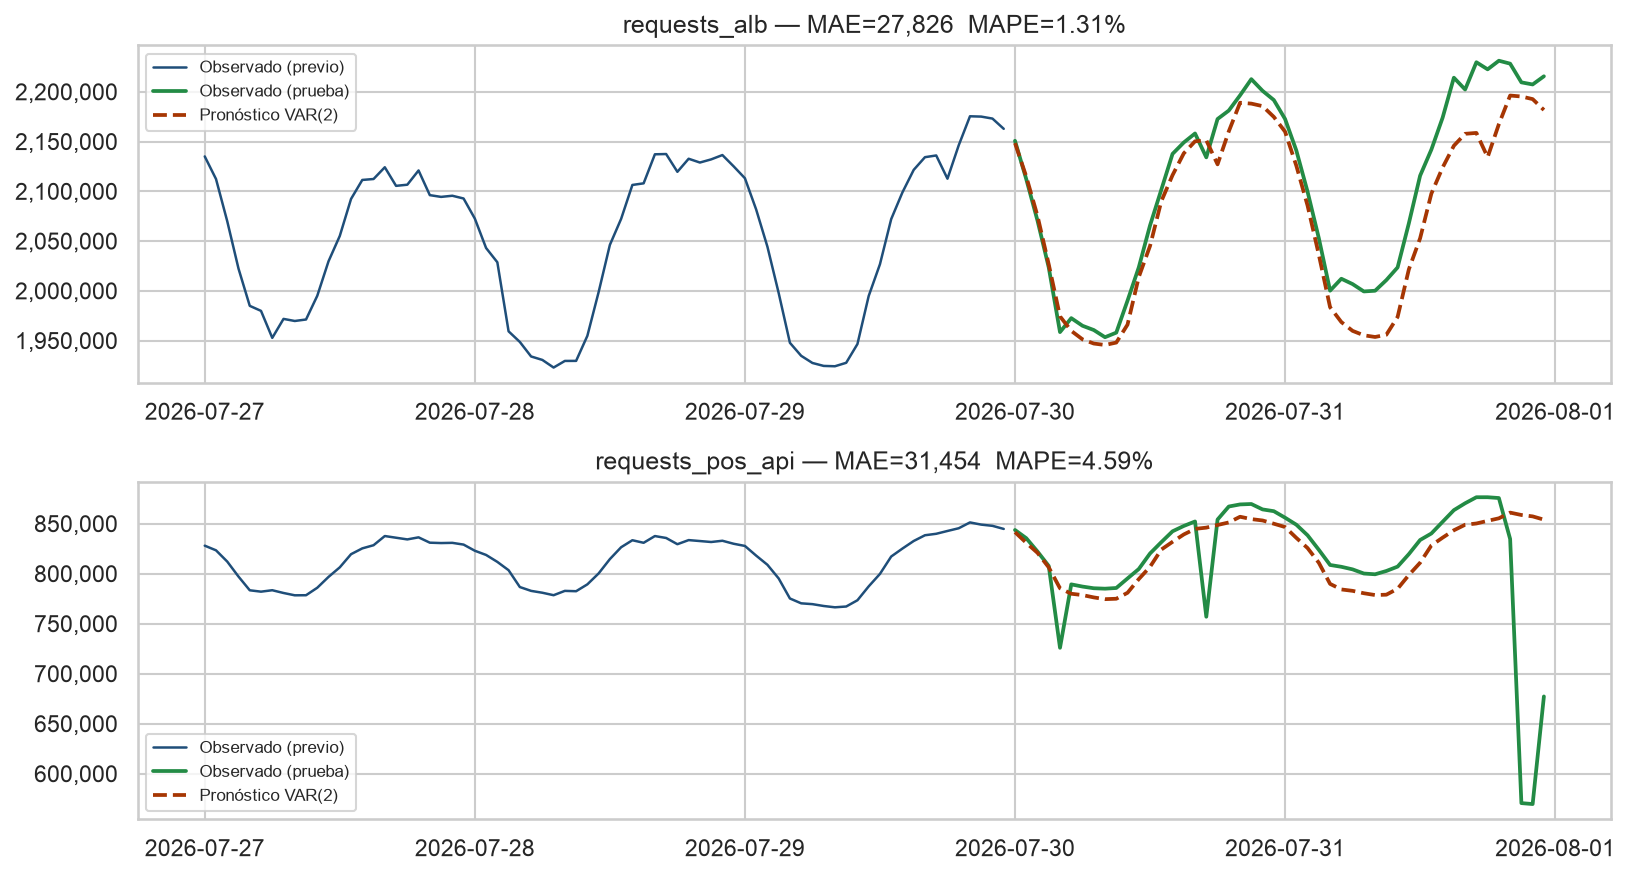
\includegraphics[width=\textwidth]{var2_pronostico.png}
\caption{Pronóstico del modelo multivariado a 48 horas, expresado en la escala original}
\label{fig:var_pron}
\end{figure}

\subsection{Impulso-respuesta y causalidad (punto 11)}

La Figura~\ref{fig:irf} presenta las funciones impulso-respuesta ortogonalizadas del modelo
adoptado. Las respuestas se extinguen con rapidez, comportamiento esperable en una especificación de orden bajo sobre series ya estacionarias.

\begin{figure}[htbp]
\centering
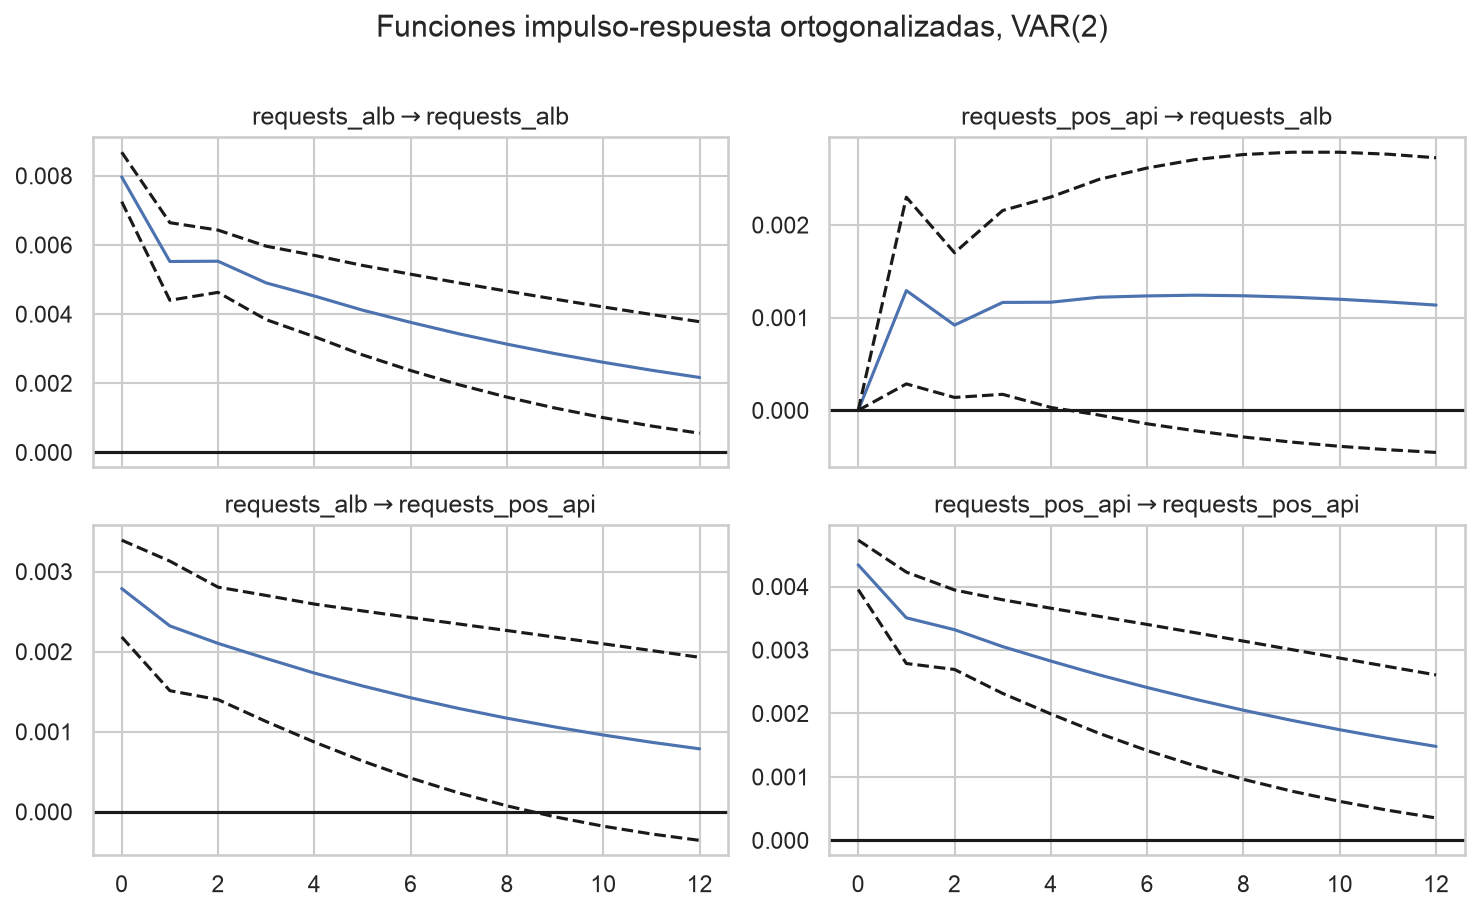
\includegraphics[width=\textwidth]{var2_irf.png}
\caption{Funciones impulso-respuesta ortogonalizadas del modelo de dos rezagos}
\label{fig:irf}
\end{figure}

La Tabla~\ref{tab:granger} presenta los contrastes de causalidad de Granger.

\begin{table}[htbp]
\centering
\caption{Contrastes de causalidad de Granger sobre el modelo adoptado}
\label{tab:granger}
\small
\begin{tabular}{llrrl}
\toprule
\textbf{Variable causante} & \textbf{Variable causada} & \textbf{$F$} & \textbf{$p$} & \textbf{Decisión al 5\,\%} \\
\midrule
Punto de venta & Balanceador & 3,554 & 0,0294 & Se rechaza $H_0$ \\
Balanceador & Punto de venta & 0,065 & 0,9369 & No se rechaza $H_0$ \\
\bottomrule
\end{tabular}
\end{table}

El resultado es unidireccional. Los rezagos de la serie de punto de venta contribuyen a
explicar la serie del balanceador, mientras que la relación inversa no alcanza
significatividad, con un valor $p$ que se aproxima a la unidad.

La interpretación admite una lectura operativa plausible: el tráfico de la interfaz de punto de venta es una porción del tráfico total que atraviesa el balanceador, de modo que un
movimiento en el primero antecede a un movimiento en el agregado. Conviene subrayar, no
obstante, la advertencia formulada en el marco teórico. La causalidad de Granger establece
precedencia temporal con contenido predictivo, no causalidad estructural. Con trece días de
solapamiento y 241 observaciones de entrenamiento, la evidencia debe considerarse indicativa.

\subsection{Estacionalidad y representación mediante SARIMA (punto 12)}

Las dos series de tráfico presentan estacionalidad diaria y quedan representadas por modelos
SARIMA con período $s = 24$. La comparación solicitada refiere a los modelos determinados con
anterioridad dentro de este mismo trabajo, esto es, a las especificaciones sin componente
estacional evaluadas en la grilla del punto 5.

Esa comparación, contenida en la Tabla~\ref{tab:sarima}, no deja lugar a dudas. En la serie del
balanceador, la omisión de la diferencia estacional eleva el error absoluto medio de 16.662 a
76.284 solicitudes, esto es, lo multiplica por más de cuatro, y el criterio de Akaike se
deteriora en más de 700 unidades. Incorporar la componente estacional es, pues, lo que decide el ajuste.

La serie de altitud, en cambio, carece de estacionalidad. El periodograma de la serie diferenciada señala un período dominante de 16,3 segundos, pero ese pico no sobrevive al contraste con la función de autocorrelación: en el rezago 16 el coeficiente llega a 0,086, por debajo de la banda de significatividad de $\pm 0{,}092$ que corresponde a una muestra de este tamaño. El pico es espurio. El episodio muestra el riesgo de leer un periodograma por separado, sin verificar sus máximos contra la autocorrelación.

La ausencia responde a la naturaleza del fenómeno: la altitud de una aeronave durante un vuelo
único obedece al plan de vuelo y a la acción del piloto automático, sin ciclo repetitivo de
período fijo. La representación adecuada es, pues, un modelo ARIMA sin componente estacional.


% ============ vii. CONCLUSIONES ============
\section{Conclusiones}

\subsection{Hallazgos principales}

El trabajo modeló tres series de naturaleza distinta y obtuvo resultados de calidad desigual,
circunstancia que conviene exponer sin uniformar.

Las dos series de tráfico presentan estacionalidad diaria inequívoca, con período de
veinticuatro horas, verificada tanto por la inspección del perfil horario como por los picos de
la función de autocorrelación en los rezagos 24, 48 y 72. Los modelos SARIMA seleccionados
alcanzan errores porcentuales del 0,79 y del 3,90 por ciento sobre un horizonte de 48 horas,
magnitudes aceptables para una serie de tráfico operativo.

Ese desempeño, sin embargo, convive con un diagnóstico de residuos desfavorable. La prueba de
Ljung-Box rechaza la incorrelación a partir del rezago 24 en la serie del balanceador, y en
todos los rezagos examinados en la serie de punto de venta. Ambos modelos dejan estructura sin
explicar, concentrada en los rezagos estacionales. Los pronósticos merecen, por lo tanto, menor
confianza que la sugerida por sus métricas de error.

La serie de altitud presenta el comportamiento opuesto. Sin componente estacional, es un proceso integrado que una sola diferencia regular vuelve
estacionario. El modelo
ARIMA$(1,1,3)$ exhibe parámetros significativos tanto individual como conjuntamente, y sus
residuos no se distinguen del ruido blanco en ningún rezago examinado. Es el único de los tres que supera el diagnóstico sin reservas.

El modelo multivariado, construido sobre las dos series de tráfico con dos rezagos, arroja una
relación de precedencia unidireccional: los rezagos de la serie de punto de venta contribuyen a
explicar la del balanceador, sin reciprocidad.

\subsection{Dos lecciones metodológicas}

Dos episodios del trabajo trascienden el resultado particular.

El primero es la selección del orden en el modelo multivariado. El criterio de Akaike sugería
24 rezagos, esto es, 98 parámetros estimados a partir de 241 observaciones. La especificación
resultante predecía peor que una de diez parámetros. Los criterios de información orientan, no dictaminan, y ante discrepancia entre ellos el desempeño fuera de muestra es el árbitro más confiable. La misma tensión reapareció, con menor intensidad, al
seleccionar el modelo estacional de la serie de punto de venta.

El segundo es de orden más elemental: una métrica mal elegida puede invertir por completo la
lectura de un resultado. El error porcentual absoluto medio del 97,20 por ciento que arrojaba
el modelo multivariado no medía su calidad sino la inadecuación de aplicar una métrica relativa
sobre una serie que oscila alrededor de cero. Expresado en la escala original, el mismo modelo
alcanza un error del 1,31 por ciento.

\subsection{Límites del trabajo}

\begin{enumerate}
\item \textbf{Tamaño muestral.} Las series de tráfico abarcan aproximadamente un mes, y la de
altitud, 457 observaciones. Ninguna admite validación mediante ventanas móviles ni evaluación
sobre múltiples horizontes independientes.

\item \textbf{Estacionalidad semanal no modelada.} El mapa de calor revela que la serie del
balanceador presenta niveles sensiblemente inferiores los días miércoles y jueves. Un período
muestral de un mes ofrece apenas cuatro repeticiones de cada día de la semana, cantidad
insuficiente para estimar una componente estacional de período 168. La autocorrelación residual detectada en el diagnóstico encaja con esa omisión.

\item \textbf{Solapamiento limitado entre las series de tráfico.} La intersección temporal
abarca trece días y 289 observaciones tras la transformación. Toda conclusión del modelo
multivariado queda condicionada por esa brevedad.

\item \textbf{Calendarios disjuntos.} La serie de altitud no participa del modelo multivariado
por corresponder a un período que no solapa con el de las restantes. La limitación es
estructural y no admite solución dentro de los datos disponibles.

\item \textbf{Alcance de la causalidad de Granger.} El contraste establece precedencia temporal
con contenido predictivo. No autoriza a afirmar que una serie cause a la otra en sentido
estructural.

\item \textbf{Un único vuelo.} Los resultados de la serie de altitud describen ese vuelo. No se
generalizan a otros vuelos ni a otras aeronaves.

\item \textbf{Normalidad de los residuos.} El contraste de Jarque-Bera rechaza la normalidad en
el modelo de la serie de altitud. Los intervalos de predicción nominales son, por eso, aproximados.
\end{enumerate}

\subsection{Líneas de trabajo futuro}

La limitación de mayor peso es la brevedad del período muestral, y corregirla destrabaría las
restantes. Un año de registro permitiría estimar la componente semanal cuya ausencia se
manifiesta en la autocorrelación residual, y ampliaría el solapamiento entre las series de
tráfico hasta un tamaño donde el modelo multivariado admitiera órdenes superiores sin
comprometer la fiabilidad.

En segundo término, el modelo del balanceador se puede simplificar. Los
parámetros de la parte regular carecen de significatividad, de modo que una especificación
$(0,1,0)\times(1,1,1)_{24}$ alcanzaría un ajuste equivalente con dos parámetros menos.

Por último, la serie de altitud ofrece una extensión natural que este trabajo no exploró: la telemetría de vuelo registra en paralelo la velocidad aerodinámica junto con la
altitud, y ambas magnitudes están vinculadas por el intercambio entre energía potencial y
cinética. Un modelo multivariado sobre ese par contaría con series perfectamente alineadas y
con una interpretación física directa de la función impulso-respuesta.


% ============ viii. REFERENCIAS BIBLIOGRÁFICAS ============
\newpage
\printbibliography[title={Referencias bibliográficas}, heading=bibintoc]

% ============ ix. APÉNDICES ============
\appendix
\section{Apéndice A. Material gráfico complementario}

Las figuras de este apéndice documentan el análisis exploratorio de las series de tráfico. Se
excluyeron del cuerpo por resultar redundantes respecto de figuras allí incluidas, o por
referir a aspectos que el trabajo no modela.

\begin{figure}[htbp]
\centering
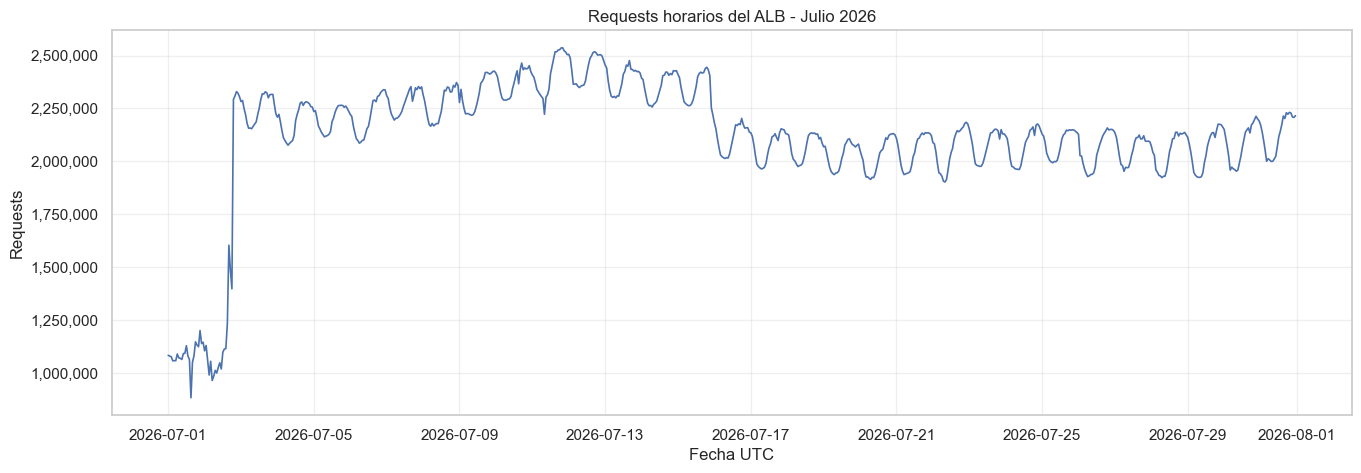
\includegraphics[width=0.85\textwidth]{alb_serie.png}
\caption{Serie horaria del balanceador de carga, análisis exploratorio}
\end{figure}

\begin{figure}[htbp]
\centering
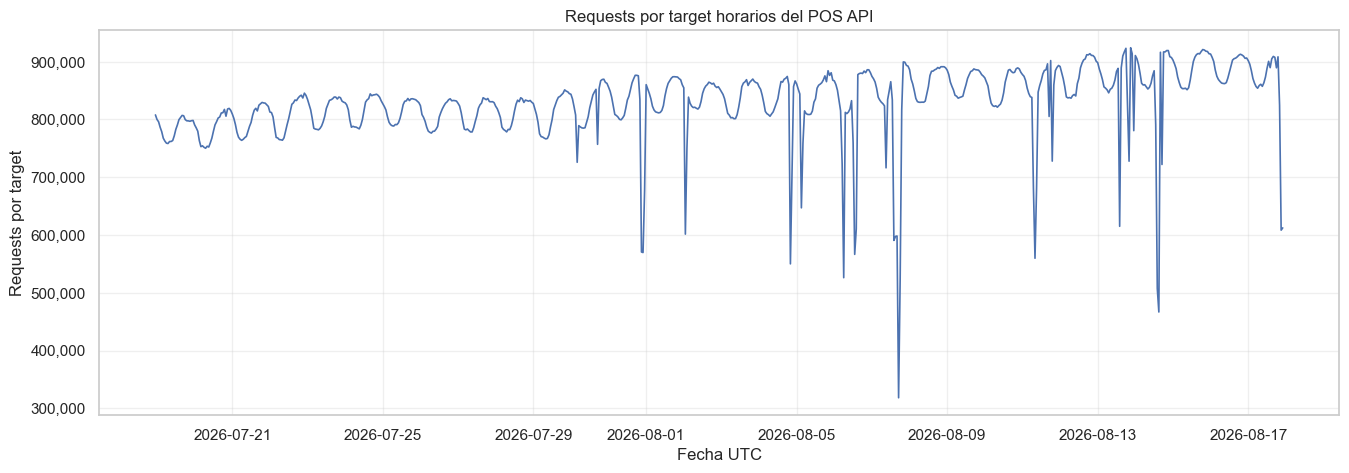
\includegraphics[width=0.85\textwidth]{pos_serie.png}
\caption{Serie horaria de punto de venta, análisis exploratorio}
\end{figure}

\begin{figure}[htbp]
\centering
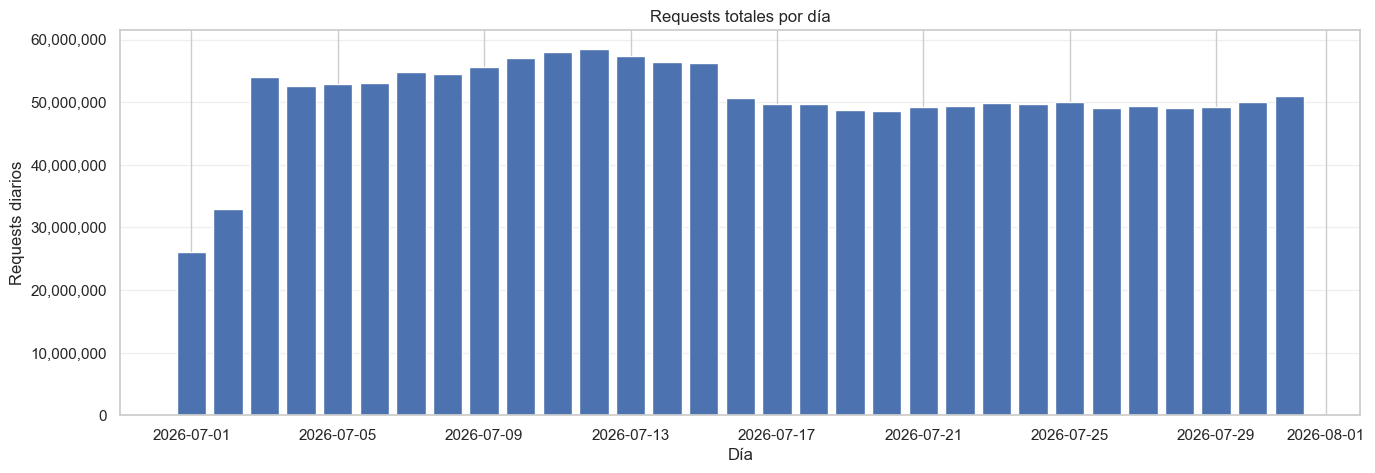
\includegraphics[width=0.85\textwidth]{alb_diaria.png}
\caption{Agregación diaria de la serie del balanceador de carga}
\end{figure}

\begin{figure}[htbp]
\centering
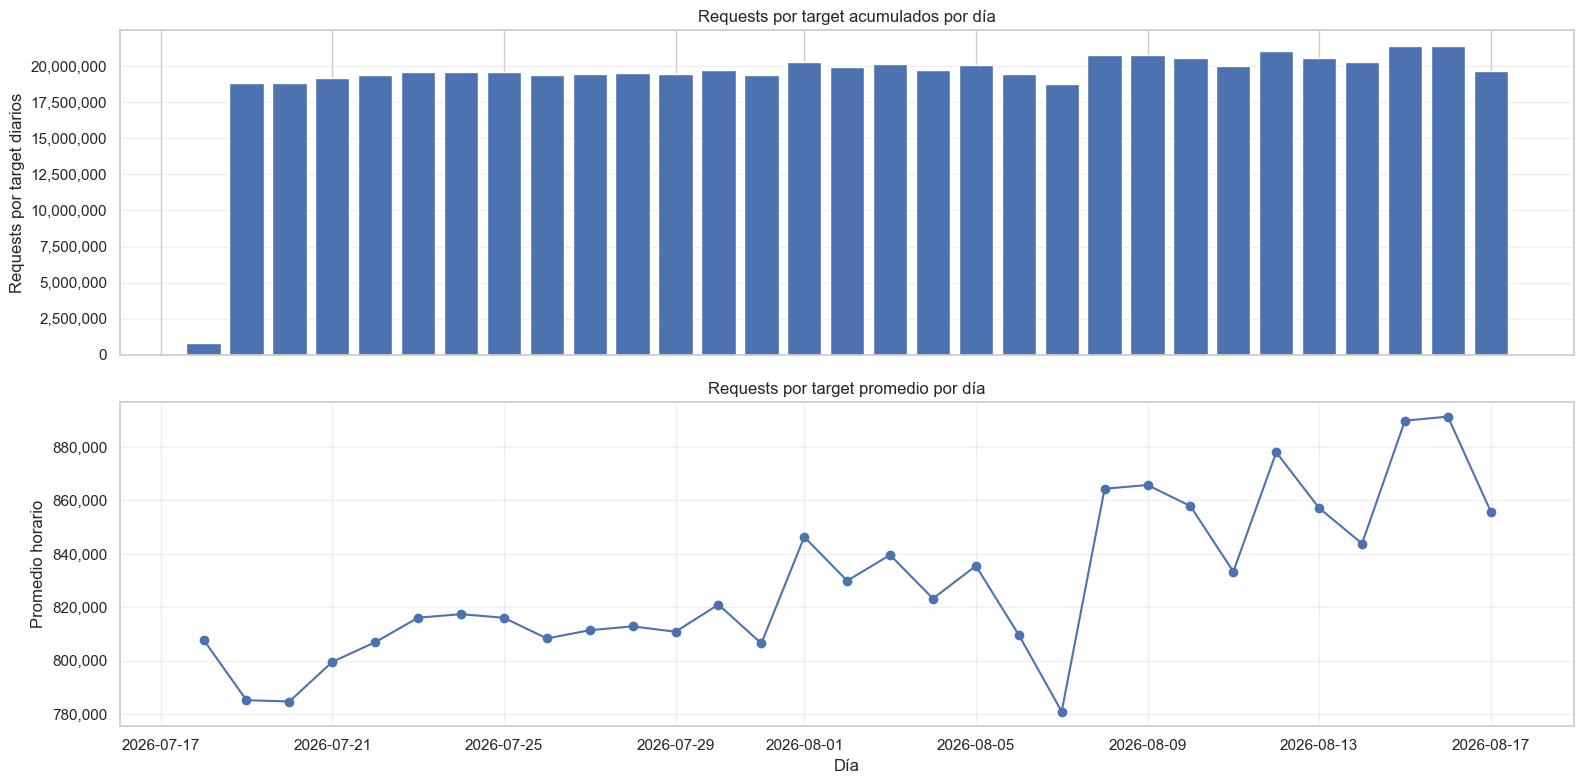
\includegraphics[width=0.85\textwidth]{pos_diaria.png}
\caption{Agregación diaria de la serie de punto de venta}
\end{figure}

\begin{figure}[htbp]
\centering
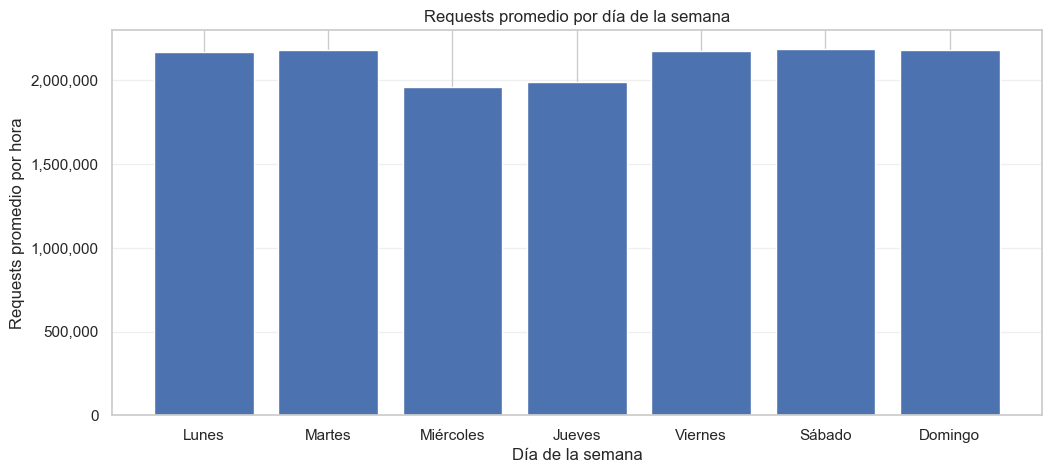
\includegraphics[width=0.85\textwidth]{alb_diasem.png}
\caption{Patrón por día de la semana, serie del balanceador de carga}
\end{figure}

\begin{figure}[htbp]
\centering
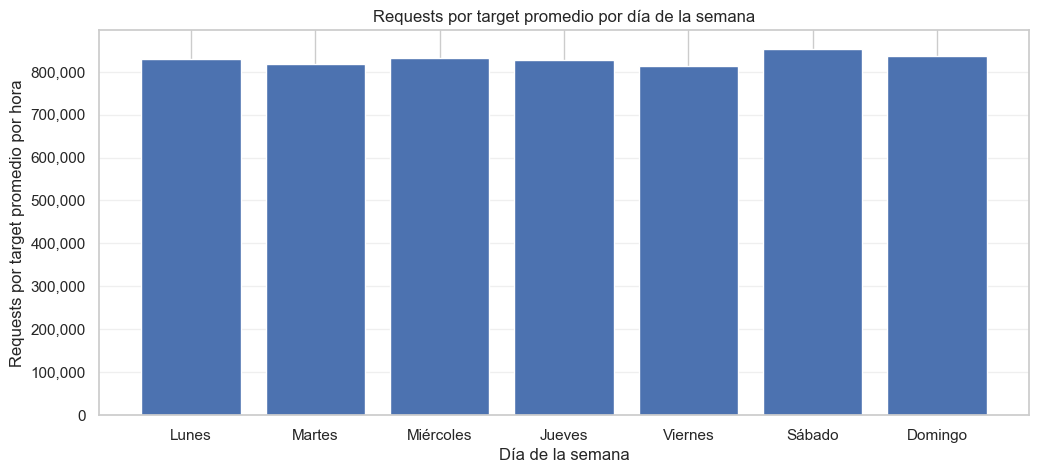
\includegraphics[width=0.85\textwidth]{pos_diasem.png}
\caption{Patrón por día de la semana, serie de punto de venta}
\end{figure}

\begin{figure}[htbp]
\centering
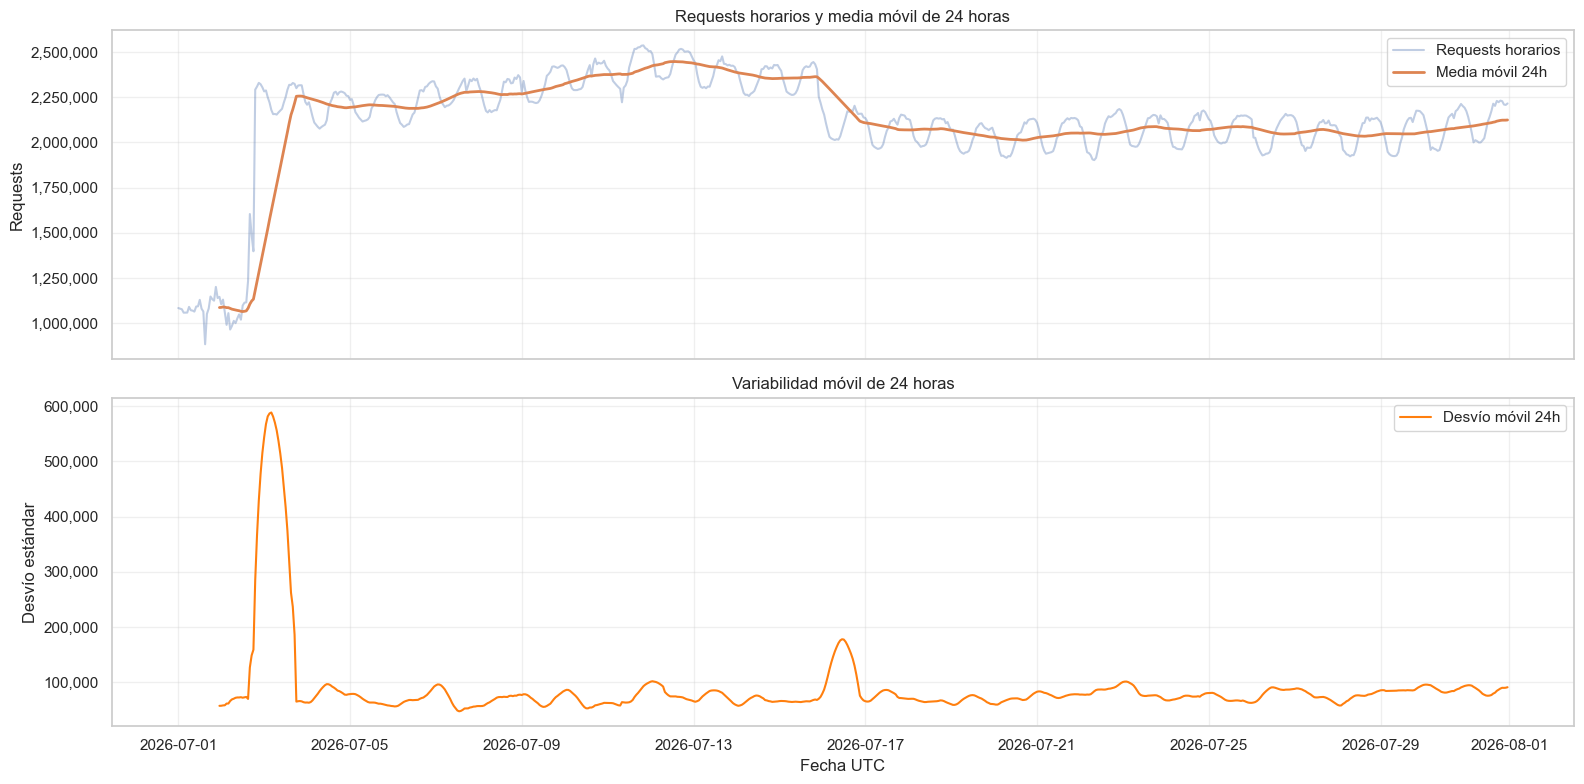
\includegraphics[width=0.85\textwidth]{alb_moviles.png}
\caption{Media y desvío estándar móviles, serie del balanceador de carga}
\end{figure}

\begin{figure}[htbp]
\centering
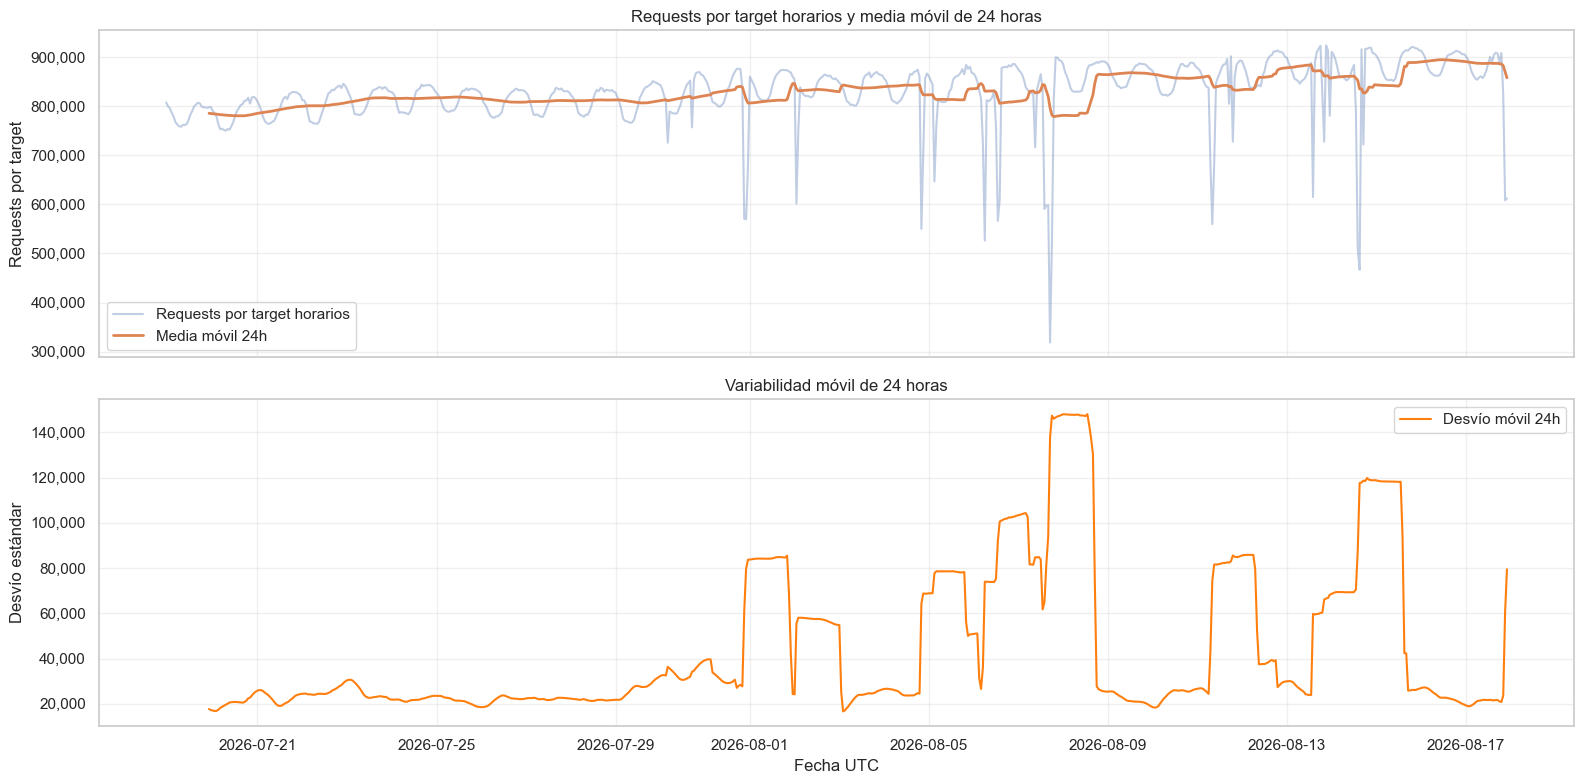
\includegraphics[width=0.85\textwidth]{pos_moviles.png}
\caption{Media y desvío estándar móviles, serie de punto de venta}
\end{figure}

\begin{figure}[htbp]
\centering
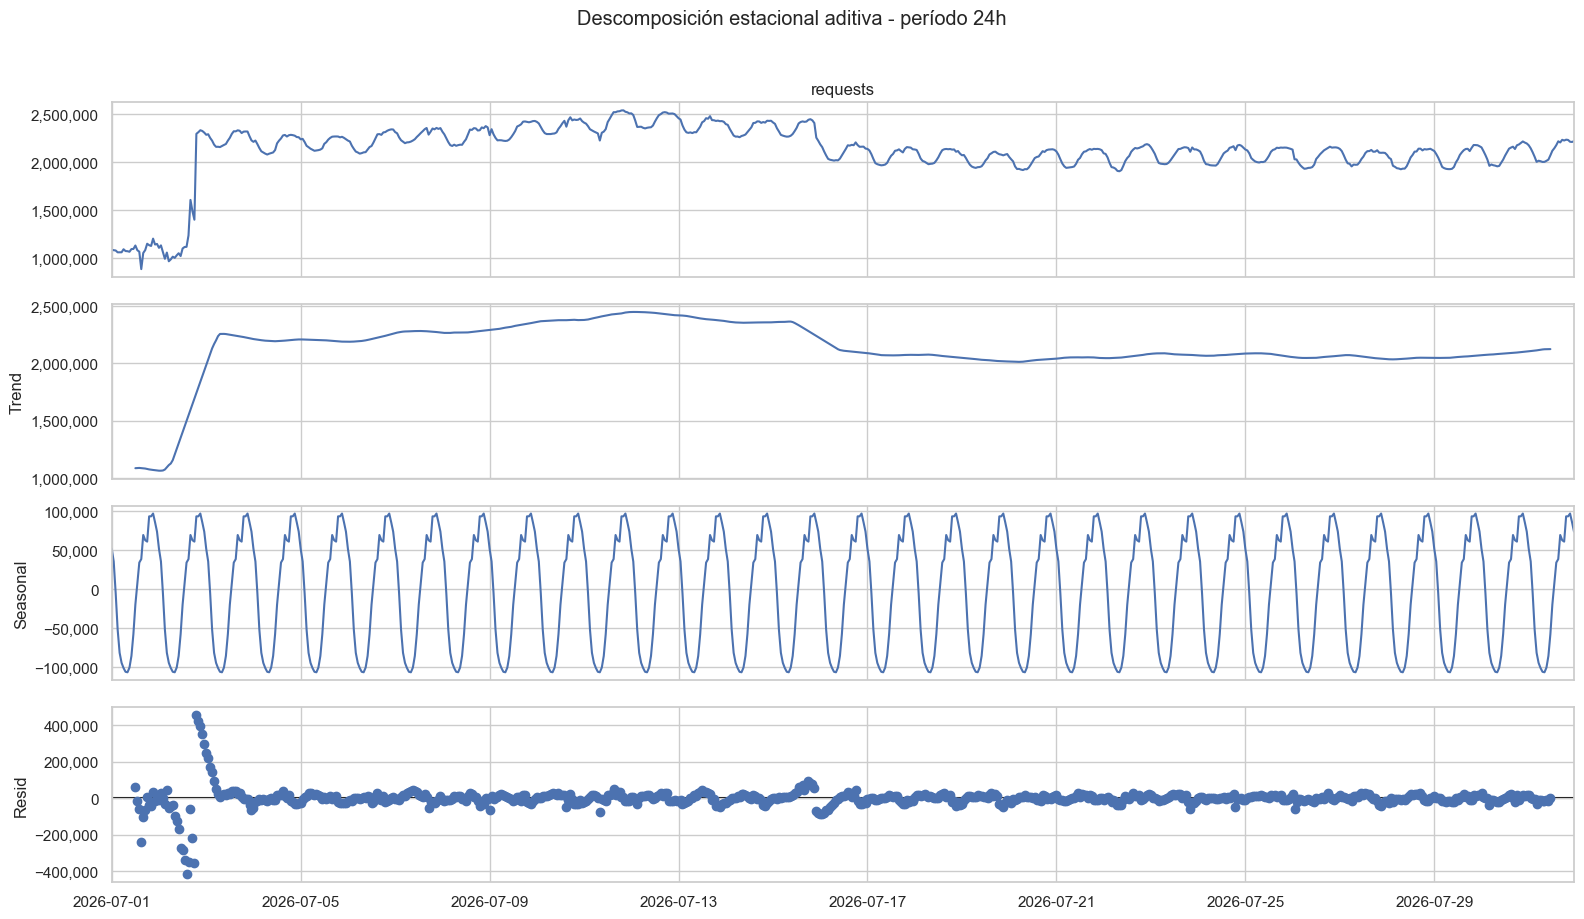
\includegraphics[width=0.85\textwidth]{alb_descomp.png}
\caption{Descomposición estacional de la serie del balanceador de carga}
\end{figure}

\begin{figure}[htbp]
\centering
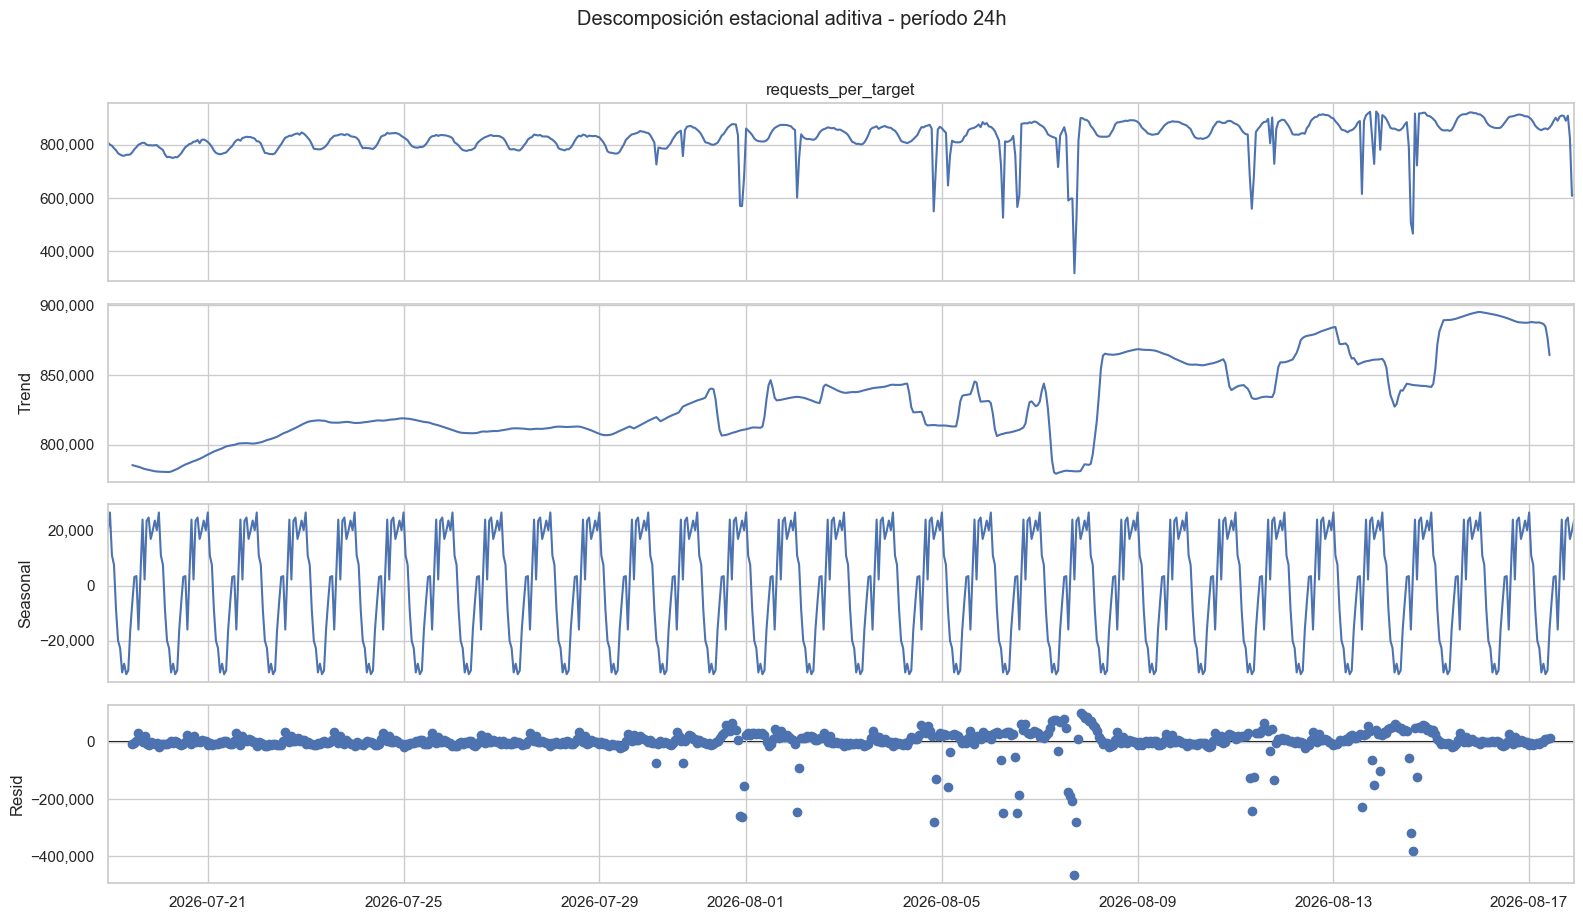
\includegraphics[width=0.85\textwidth]{pos_descomp.png}
\caption{Descomposición estacional de la serie de punto de venta}
\end{figure}

\begin{figure}[htbp]
\centering
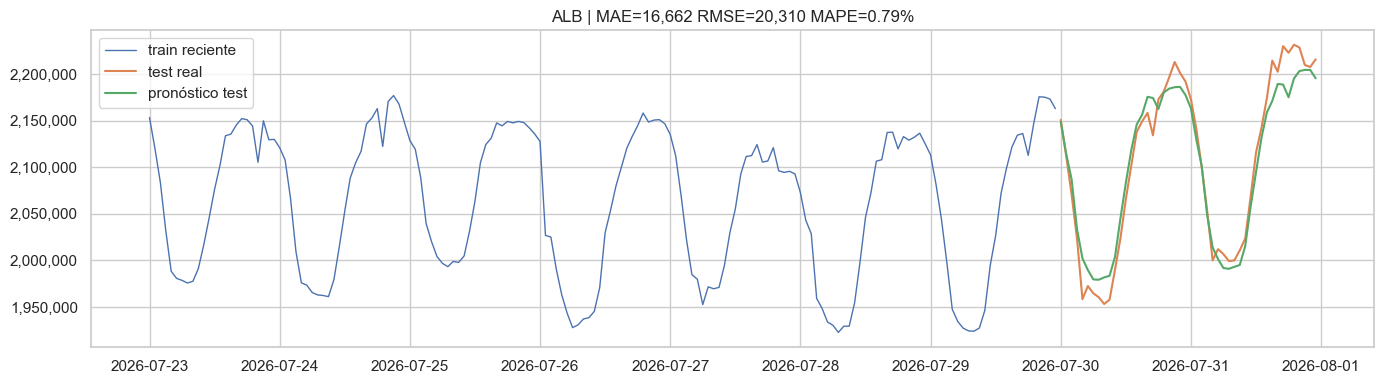
\includegraphics[width=0.85\textwidth]{trafico_traintest_1.png}
\caption{Ajuste sobre el conjunto de prueba, serie del balanceador de carga}
\end{figure}

\begin{figure}[htbp]
\centering
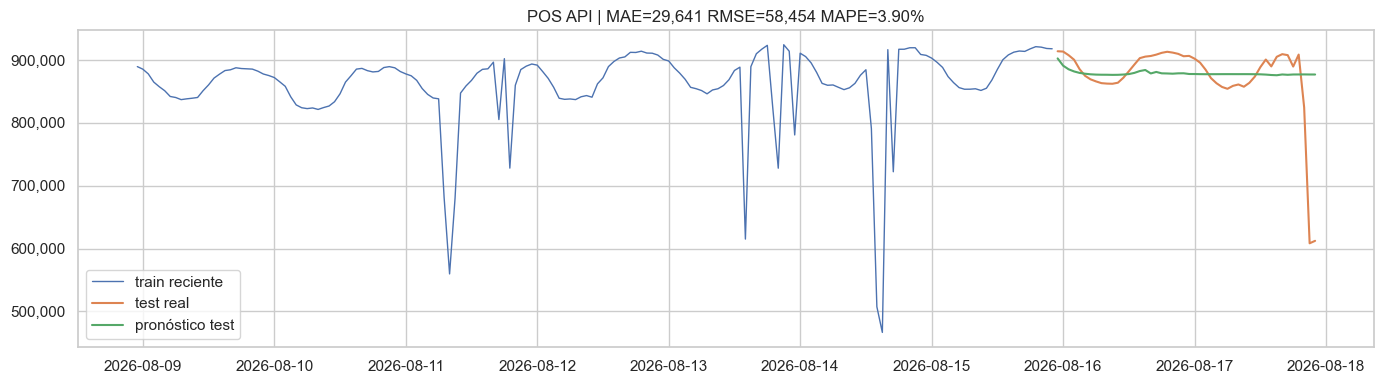
\includegraphics[width=0.85\textwidth]{trafico_traintest_2.png}
\caption{Ajuste sobre el conjunto de prueba, serie de punto de venta}
\end{figure}

\section{Apéndice B. Rutinas de cómputo}

\subsection*{Construcción de la serie de altitud}

La rutina siguiente extrae la altitud del registro binario de telemetría, la lleva a una grilla
regular de un segundo y aísla el tramo contiguo más extenso en vuelo.

\begin{lstlisting}
def leer_altitud(ruta):
    """Extrae la altitud relativa, en metros, de un registro MAVLink."""
    conexion = mavutil.mavlink_connection(ruta)
    registros = []
    while True:
        mensaje = conexion.recv_match(type="GLOBAL_POSITION_INT")
        if mensaje is None:
            break
        registros.append((mensaje._timestamp, mensaje.relative_alt / 1000.0))
    crudo = pd.DataFrame(registros, columns=["timestamp", "altitud_m"])
    crudo["timestamp"] = pd.to_datetime(crudo["timestamp"], unit="s")
    return crudo.set_index("timestamp")["altitud_m"]


def bloque_contiguo_mas_largo(mascara):
    """Indices de inicio y fin del tramo contiguo mas largo que cumple la mascara."""
    mejor_inicio, mejor_largo = 0, 0
    inicio = None
    for posicion, activo in enumerate(mascara):
        if activo and inicio is None:
            inicio = posicion
        elif not activo and inicio is not None:
            if posicion - inicio > mejor_largo:
                mejor_inicio, mejor_largo = inicio, posicion - inicio
            inicio = None
    if inicio is not None and len(mascara) - inicio > mejor_largo:
        mejor_inicio, mejor_largo = inicio, len(mascara) - inicio
    return mejor_inicio, mejor_inicio + mejor_largo
\end{lstlisting}

\subsection*{Representación conjunta de las tres funciones}

\begin{lstlisting}
def graficar_fas_fac_facp(datos, titulo, rezagos=40):
    """Grafica autocovarianza, autocorrelacion y parcial en una sola figura."""
    figura, ejes = plt.subplots(1, 3, figsize=(13, 3.4))
    autocovarianza = sm.tsa.acovf(datos, nlag=rezagos, fft=True)
    ejes[0].stem(range(len(autocovarianza)), autocovarianza, basefmt=" ")
    ejes[0].set_title("FAS - autocovarianza")
    plot_acf(datos, lags=rezagos, ax=ejes[1], title="FAC - autocorrelacion")
    plot_pacf(datos, lags=rezagos, ax=ejes[2], method="ywm",
              title="FACP - autocorrelacion parcial")
    figura.suptitle(titulo, y=1.05)
    plt.tight_layout()
    plt.show()
\end{lstlisting}

\subsection*{Comparación de especificaciones del modelo multivariado}

La rutina siguiente evalúa cada orden de rezagos e invierte la transformación antes de calcular
las métricas, de modo que el error quede expresado en la escala original.

\begin{lstlisting}
def evaluar(p, entrenamiento, prueba, log_original, alineadas, horizonte):
    resultado = VAR(entrenamiento).fit(p)
    pronostico = pd.DataFrame(
        resultado.forecast(entrenamiento.values[-p:], horizonte),
        index=prueba.index, columns=prueba.columns)
    filas = []
    for columna in prueba.columns:
        historico = log_original[columna].copy()
        prediccion = []
        for i, t in enumerate(prueba.index):
            base = historico.loc[t - pd.Timedelta(hours=24)]
            valor = base + pronostico[columna].iloc[i]
            historico.loc[t] = valor
            prediccion.append(valor)
        estimado = np.expm1(np.array(prediccion))
        real = alineadas[columna].reindex(prueba.index).to_numpy()
        filas.append({
            "rezagos": p,
            "serie": columna,
            "MAE": np.mean(np.abs(estimado - real)),
            "RMSE": np.sqrt(np.mean((estimado - real) ** 2)),
            "MAPE": np.mean(np.abs((estimado - real) / real)) * 100,
        })
    return filas
\end{lstlisting}


\end{document}
